\documentclass[12pt,a4paper]{article}
\usepackage[a4paper, margin=0.8in, headheight=14pt]{geometry}
\usepackage{fontspec}
\usepackage{unicode-math}
\setmainfont{TeX Gyre Pagella}
\setmonofont[Scale=0.88]{TeX Gyre Cursor}
\setmathfont{Latin Modern Math}
\usepackage{xcolor}
\usepackage{colortbl}
\usepackage{titlesec}
\usepackage{enumitem}
\usepackage{tabularx}
\usepackage{booktabs}
\usepackage{array}
\usepackage{amsmath}
\usepackage{tikz}
\usetikzlibrary{shapes.geometric, arrows.meta, positioning, calc, fit, decorations.pathreplacing, decorations.pathmorphing}
\usepackage{tcolorbox}
\tcbuselibrary{skins, breakable}
\usepackage{hyperref}
\usepackage{fancyhdr}
\usepackage{graphicx}
\usepackage{microtype}
\hyphenpenalty=10000
\exhyphenpenalty=10000
\sloppy
\usepackage{caption}
\usepackage{setspace}
\usepackage{multirow}
\usepackage{tocloft}
\newcommand{\Q}[1]{\textbf{#1}\par\noindent\ignorespaces}
\definecolor{myred}{RGB}{196,30,58}
\definecolor{mydark}{RGB}{30,30,50}
\definecolor{mygreen}{RGB}{14,120,80}
\definecolor{myteal}{RGB}{0,130,140}
\definecolor{myamber}{RGB}{180,100,0}
\definecolor{mypurple}{RGB}{100,30,160}
\definecolor{mygray}{RGB}{246,247,249}
\definecolor{mgframe}{RGB}{180,185,200}
\definecolor{watermark}{RGB}{145,150,170}
\definecolor{hdrred}{RGB}{250,232,235}
\definecolor{hdrgreen}{RGB}{220,244,233}
\definecolor{hdrteal}{RGB}{220,242,244}
\definecolor{hdramber}{RGB}{253,242,215}
\definecolor{hdrpurple}{RGB}{238,228,255}
\definecolor{hdrgray}{RGB}{238,240,245}
\definecolor{rowalt}{RGB}{250,251,253}

\titleformat{\section}{\large\bfseries\color{myred}}{\thesection.}{0.5em}{}[\vspace{1pt}{\color{myred}\rule{\linewidth}{0.8pt}}]
\titleformat{\subsection}{\normalsize\bfseries\color{myteal}}{\thesubsection}{0.5em}{}
\titlespacing*{\section}{0pt}{18pt}{7pt}
\titlespacing*{\subsection}{0pt}{11pt}{4pt}
\setlength{\parindent}{0pt}
\setlength{\parskip}{4pt}
\renewcommand{\cfttoctitlefont}{\large\bfseries\color{myred}}
\renewcommand{\cftaftertoctitle}{\par\noindent{\color{myred}\rule{\linewidth}{0.8pt}}}
\setlength{\cftbeforetoctitleskip}{0pt}
\setlength{\cftaftertoctitleskip}{6pt}
\renewcommand{\cftsecfont}{\normalsize\bfseries\color{mydark}}
\renewcommand{\cftsecpagefont}{\normalsize\bfseries\color{mydark}}
\renewcommand{\cftsecleader}{\cftdotfill{\cftdotsep}}
\setlength{\cftbeforesecskip}{7pt}
\renewcommand{\cftsubsecfont}{\small\color{mydark}}
\renewcommand{\cftsubsecpagefont}{\small\color{mydark}}
\setlength{\cftbeforesubsecskip}{3pt}
\setlength{\cftsubsecindent}{1.4em}
\renewcommand{\cftpartfont}{\normalsize\bfseries\color{myteal}}
\renewcommand{\cftpartpagefont}{\normalsize\bfseries\color{myteal}}
\setlength{\cftbeforepartskip}{14pt}
\renewcommand{\arraystretch}{1.45}
\setlength{\tabcolsep}{6pt}
\arrayrulecolor{mydark}
\newcolumntype{B}[1]{>{\small\bfseries\raggedright\arraybackslash}m{#1}}
\newcolumntype{C}[1]{>{\centering\arraybackslash}m{#1}}
\newcolumntype{Y}{>{\small\raggedright\arraybackslash}X}
\renewcommand{\tabularxcolumn}[1]{m{#1}}
\newcommand{\currmodule}{Module 1}
\pagestyle{fancy}
\fancyhf{}
\fancyhead[L]{\small\color{myred}\textbf{OE-EC604B}\;\color{mydark}--- Operating System}
\fancyhead[R]{\small\color{myteal}\textbf{\currmodule\ Notes}}
\fancyfoot[C]{\small\color{mydark}\thepage}
\fancyfoot[R]{\small\color{watermark}\textit{\copyright\ Biraj}}
\renewcommand{\headrulewidth}{0.5pt}
\renewcommand{\footrulewidth}{0.3pt}

\hypersetup{colorlinks=true, linkcolor=myteal, urlcolor=myteal,
  pdfauthor={Biraj Sarkar},
  pdftitle={OE-EC604B --- Combined Notes}}

\tcbset{
  tikzbox/.style={
    colback=mygray, colframe=mgframe, boxrule=0.6pt, arc=4pt,
    left=8pt, right=8pt, top=6pt, bottom=6pt,
    colbacktitle=mgframe, coltitle=mydark,
    fonttitle=\small\bfseries
  },
  defbox/.style={
    colback=hdrgreen, colframe=mygreen, boxrule=0.8pt, arc=4pt,
    left=9pt, right=9pt, top=6pt, bottom=6pt,
    colbacktitle=mygreen, coltitle=white,
    fonttitle=\small\bfseries
  },
  formulabox/.style={
    colback=hdrteal, colframe=myteal, boxrule=0.8pt, arc=4pt,
    left=9pt, right=9pt, top=7pt, bottom=7pt,
    colbacktitle=myteal, coltitle=white,
    fonttitle=\small\bfseries
  },
  examplebox/.style={
    colback=hdramber, colframe=myamber, boxrule=0.8pt, arc=4pt,
    left=9pt, right=9pt, top=6pt, bottom=6pt,
    colbacktitle=myamber, coltitle=white,
    fonttitle=\small\bfseries
  },
  masonbox/.style={
    colback=hdrpurple, colframe=mypurple, boxrule=0.8pt, arc=4pt,
    left=9pt, right=9pt, top=6pt, bottom=6pt,
    colbacktitle=mypurple, coltitle=white,
    fonttitle=\small\bfseries
  },
  exambox/.style={
    colback=hdrpurple, colframe=mypurple, boxrule=1pt, arc=5pt,
    left=10pt, right=10pt, top=8pt, bottom=8pt,
    colbacktitle=mypurple, coltitle=white,
    fonttitle=\bfseries,
    breakable, title after break={\textbf{Frequently Asked / Viva Questions (contd.)}}}
}
\tcbset{after={\color{black}}}

\tikzset{
  block/.style={rectangle, draw=myteal, fill=hdrteal,
    text width=2.4cm, align=center, minimum height=0.95cm,
    font=\small, rounded corners=3pt, line width=0.7pt},
  redblock/.style={rectangle, draw=myred, fill=hdrred,
    text width=2.4cm, align=center, minimum height=0.95cm,
    font=\small, rounded corners=3pt, line width=0.7pt},
  greenblock/.style={rectangle, draw=mygreen, fill=hdrgreen,
    text width=2.4cm, align=center, minimum height=0.95cm,
    font=\small, rounded corners=3pt, line width=0.7pt},
  amberblock/.style={rectangle, draw=myamber, fill=hdramber,
    text width=2.4cm, align=center, minimum height=0.95cm,
    font=\small, rounded corners=3pt, line width=0.7pt},
  purpblock/.style={rectangle, draw=mypurple, fill=hdrpurple,
    text width=2.4cm, align=center, minimum height=0.95cm,
    font=\small, rounded corners=3pt, line width=0.7pt},
  sumjunc/.style={circle, draw=myamber, fill=hdramber,
    minimum size=0.62cm, font=\small, line width=0.8pt},
  arrow/.style={-Stealth, thick, color=mydark},
  redarrow/.style={-Stealth, thick, color=myred},
  line/.style={thick, color=mydark}
}

\newcommand{\modulestart}[2]{%
  \clearpage
  \renewcommand{\currmodule}{Module #1}%
  \phantomsection
  \addcontentsline{toc}{part}{Module #1: #2}%
  \setcounter{section}{0}%
  \begin{center}
    \vspace*{1.0cm}
    {\Huge\bfseries\color{myred} Module #1}\\[10pt]
    {\Large\bfseries\color{mydark} #2}\\[10pt]
    {\color{myred}\rule{0.55\linewidth}{1.2pt}}
  \end{center}
  \vspace{14pt}
}
\begin{document}

\thispagestyle{empty}
\vspace*{1.0cm}
\begin{center}
  {\Huge\bfseries\color{myred} OE-EC604B}\\[10pt]
  {\LARGE\bfseries\color{mydark} Operating System}\\[20pt]
  {\color{myred}\rule{0.7\linewidth}{1.5pt}}\\[18pt]
  {\Large\color{myteal}\textbf{Combined Module Notes}}\\[8pt]
  {\large\color{mydark} Modules 1 -- 9}\\[40pt]
  {\normalsize\color{mydark} Semester VI \quad$\bullet$\quad 3L:0T:0P \quad$\bullet$\quad 3 Credits}\\[12pt]
  {\normalsize\color{mydark} CGEC \;$|$\; B.Tech ECE (2023--27)}\\[6pt]
  {\normalsize\color{mydark}\textit{Biraj Sarkar}}
\end{center}
\vspace{1.0cm}
\begin{center}
  \begin{tcolorbox}[colback=mygray, colframe=mgframe, boxrule=0.5pt, arc=3pt, width=0.85\linewidth]
    \centering\small\color{mydark}
    \textbf{Disclaimer / Study Guide Notice:}\\
    These are condensed \textbf{Short Notes} focusing on core theory, key formulas, block/circuit diagrams, and standard viva Q\&As for university exam revision. Exhaustive numerical practice problems and derivation edge cases are not covered. This serves as a quick-revision reference guide for students.
  \end{tcolorbox}
\end{center}
\vfill
\begin{center}{\small\color{watermark}\textit{Exam-Ready Notes}}\end{center}
\clearpage

\hypersetup{linkcolor=mydark}
\tableofcontents
\hypersetup{linkcolor=myteal}
\clearpage

% -- Module 1 -----------------------------------------------------------------
\modulestart{1}{Operating System and Functions}

\section{Operating System and Functions}
% ===============================================================================

An \textbf{Operating System (OS)} acts as an intermediary between the user of a computer and the computer hardware. Its primary goals are to make the computer system convenient to use and to execute user programs in an efficient manner.

\subsection{Conceptual View of a Computer System}

\begin{tcolorbox}[tikzbox, title={Four Layers of a Computer System}]
\centering
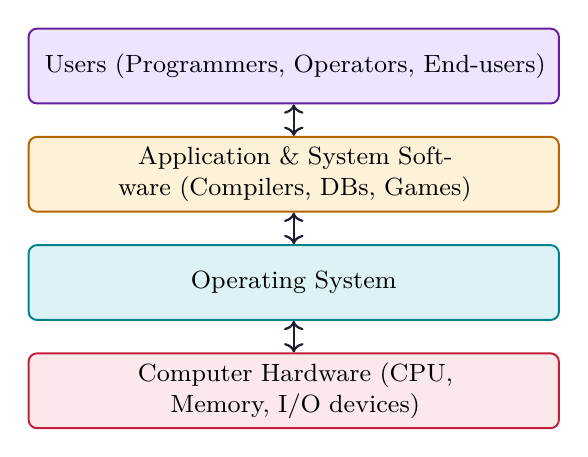
\begin{tikzpicture}[node distance=0.8cm, thick, font=\small]
  \node[block, text width=6.5cm, fill=hdrpurple, draw=mypurple] (users) {Users (Programmers, Operators, End-users)};
  \node[block, text width=6.5cm, fill=hdramber, draw=myamber, below=0.4cm of users] (apps) {Application \& System Software (Compilers, DBs, Games)};
  \node[block, text width=6.5cm, fill=hdrteal, draw=myteal, below=0.4cm of apps] (os) {Operating System};
  \node[block, text width=6.5cm, fill=hdrred, draw=myred, below=0.4cm of os] (hw) {Computer Hardware (CPU, Memory, I/O devices)};

  \draw[arrow, <->] (users) -- (apps);
  \draw[arrow, <->] (apps) -- (os);
  \draw[arrow, <->] (os) -- (hw);
\end{tikzpicture}
\end{tcolorbox}

\subsection{Core Functions of an Operating System}

\begin{tcolorbox}[defbox, title={\textbf{Definition: Operating System}}]
An \textbf{Operating System} is a system software that manages computer hardware, software resources, and provides common services for computer programs.
\end{tcolorbox}

From an engineering perspective, the functions of an OS can be classified into five major resource management categories:\par\noindent
\begin{tabularx}{\linewidth}{|B{3.2cm}|Y|}
\hline
\textbf{Function} & \textbf{\color{myteal}Description and Key Responsibilities} \\
\hline
\textbf{Process Management} & Creation, execution, scheduling, synchronization, and termination of active processes. \\
\hline
\textbf{Memory Management} & Tracking free and allocated memory spaces, page mapping, swapping, and virtual memory allocation. \\
\hline
\textbf{File System Management} & Organising directories, files, mapping files to secondary storage, and access controls. \\
\hline
\textbf{Device (I/O) Management} & Buffering, caching, spooling, device drivers, and disk head scheduling. \\
\hline
\textbf{Protection \& Security} & Controlling user access, authentication, preventing unauthorized access, and threat mitigation. \\
\hline
\end{tabularx}

% ===============================================================================
\section{Evolution of Operating Systems}
% ===============================================================================

Operating systems have evolved from simple manual job setups on mainframes to complex distributed real-time systems.

\subsection{Batch Processing Systems}
Early mainframes used a batch system where the user had no direct access to the machine. Jobs were prepared offline on punched cards and grouped into batches by an operator.
\begin{itemize}[leftmargin=*, itemsep=3pt]
  \item \textbf{Working Principle:} A program called the \textbf{resident monitor} stayed in memory, automatically loading and running subsequent jobs from the tape/card reader one after another.
  \item \textbf{Drawback:} No interactive user control, and extremely low CPU utilization due to the speed disparity between mechanical I/O devices (slow) and electronic CPU (fast).
\end{itemize}

\subsection{Interactive \& Multi-Programmed Systems}
To overcome batch limitations, multi-programmed systems kept multiple jobs in memory simultaneously. When one job had to wait for I/O, the OS switched CPU execution to another job.
\begin{itemize}[leftmargin=*, itemsep=3pt]
  \item \textbf{Interactive Systems:} Allowed direct communication between the user and system via a keyboard/terminal, giving immediate feedback.
\end{itemize}

\subsection{Time-Sharing Systems}
Time-sharing is a logical extension of multi-programming that provides fast interactive response times.
\begin{itemize}[leftmargin=*, itemsep=3pt]
  \item \textbf{Working Principle:} The CPU executes multiple jobs by switching among them extremely fast using a fixed time quantum (slice). Each user gets a dedicated, albeit small, fraction of the CPU time, giving the illusion of a dedicated machine.
  \item \textbf{Key Goal:} Minimizing \textbf{response time} for multiple simultaneous users.
\end{itemize}

% ===============================================================================
\section{Specialized Operating Systems}
% ===============================================================================

\subsection{Real-Time Systems (RTS)}
A \textbf{Real-Time Operating System (RTOS)} is used when rigid time requirements are placed on the operation of a processor or the flow of data. The correctness of an RTOS depends not only on the logical result of computation but also on the \textbf{time} at which it is delivered.

\begin{tcolorbox}[defbox, title={\textbf{Definition: Real-Time Systems}}]
A \textbf{Real-Time System} guarantees that critical tasks are completed within strict, specified time constraints (deadlines).
\end{tcolorbox}

Real-time systems are classified into two categories based on the severity of missing deadlines:\par\noindent
\begin{tabularx}{\linewidth}{|B{3.2cm}|Y|Y|}
\hline
\textbf{Feature} & \textbf{\color{myred}Hard Real-Time System} & \textbf{\color{myteal}Soft Real-Time System} \\
\hline
\textbf{Deadline Violation} & Catastrophic system failure. & Performance degradation only. \\
\hline
\textbf{Tolerance} & Zero tolerance. Deadlines must be met. & Occasional misses are tolerated. \\
\hline
\textbf{Memory Support} & Virtual memory is usually disabled. & Virtual memory is allowed. \\
\hline
\textbf{Examples} & pacemakers, missile guidance, airbags. & Video streaming, online gaming, audio. \\
\hline
\end{tabularx}

\subsection{Multi-Threading Systems}
A \textbf{thread} (or lightweight process) is a basic unit of CPU utilization. In a multi-threading operating system, a single process can spawn multiple concurrent threads of execution, all sharing the same code segment, data segment, and system resources, but having their own thread ID, program counter, register set, and stack.

\begin{itemize}[leftmargin=*, itemsep=3pt]
  \item \textbf{Benefits:} Responsiveness (non-blocking UI), resource sharing (threads share process memory), economy (context switching is faster than process creation), and multicore utilization.
\end{itemize}

\newpage
% ===============================================================================
% MANDATORY QUICK REVISION PAGE
% ===============================================================================
\begin{center}
  {\large\bfseries\color{myred} Quick Revision --- Module 1}\\[3pt]
  {\small\color{mydark} Introduction to Operating Systems $|$ OE-EC604B}
\end{center}
\noindent{\color{myred}\rule{\linewidth}{1.2pt}}
\vspace{4pt}

\begin{tcolorbox}[formulabox, title={\textbf{Key Evolution Properties at a Glance}}]
\renewcommand{\arraystretch}{1.3}
\begin{tabularx}{\linewidth}{B{3.8cm} X}
Batch OS & Low CPU utilization, high turnaround time, offline execution. \\[4pt]
Multiprogramming & High CPU utilization, keeps multiple jobs in memory, switches on I/O. \\[4pt]
Time-Sharing & Fixed time-slice (quantum), interactive, minimizes response time. \\[4pt]
Hard Real-Time & Strict deadlines, safety-critical, no virtual memory, predictable delay. \\[4pt]
Soft Real-Time & Best-effort deadlines, priority scheduling, virtual memory allowed.
\end{tabularx}
\end{tcolorbox}

\begin{tcolorbox}[defbox, title={\textbf{One-Line Definitions}}]
\begin{itemize}[leftmargin=*, itemsep=2.5pt, topsep=0pt]
  \item \textbf{Operating System:} System software managing hardware resources and acting as a user-hardware interface.
  \item \textbf{Spooling:} Simultaneous Peripheral Operations On-Line; placing I/O data in disk buffer to speed up batch execution.
  \item \textbf{Multiprogramming:} OS technique running multiple jobs concurrently to maximize CPU utilization.
  \item \textbf{Time-Sharing:} Preemptive multiprogramming where CPU switches quickly between users using a time slice.
  \item \textbf{Real-Time OS:} Time-bound operating system designed for deterministic response times and deadlines.
  \item \textbf{Hard Real-Time:} OS where missing a single task deadline results in catastrophic system failure.
  \item \textbf{Soft Real-Time:} OS where deadlines are preferred but occasional misses do not cause system failure.
  \item \textbf{Thread:} A lightweight process representing a single sequential flow of control within a process.
  \item \textbf{Resident Monitor:} Early batch supervisor program residing in memory to load jobs automatically.
\end{itemize}
\end{tcolorbox}

\begin{tcolorbox}[exambox, title={\textbf{Frequently Asked / Viva Questions}}]
\begin{enumerate}[topsep=0pt, label=\textbf{Q\arabic*.}, itemsep=5pt]
  \item \Q{What are the primary objectives of an operating system?}
    To make the computer system convenient to use for the user, and to allocate and manage the hardware resources (CPU, memory, devices) in an efficient and fair manner.
  \item \Q{Explain the difference between Multiprogramming and Multiprocessing.}
    Multiprogramming keeps multiple processes in main memory simultaneously on a single CPU, switching between them to keep the CPU busy. Multiprocessing involves a computer system with two or more physical CPUs executing processes in parallel.
  \item \Q{What is spooling? How does it differ from buffering?}
    Spooling uses the disk as a large buffer to store incoming/outgoing jobs and data for slow peripheral devices (like printers), enabling concurrent CPU processing. Buffering is a temporary storage area in main memory used during I/O transfers to smooth out speed differences.
  \item \Q{Differentiate between Hard Real-Time and Soft Real-Time systems.}
    Hard Real-Time systems have strict, non-negotiable deadlines where any failure causes catastrophic system collapse (e.g., flight controller). Soft Real-Time systems treat deadlines as highly desirable but tolerate occasional misses without failure (e.g., video player).
  \item \Q{What is the time-sharing concept? Which scheduling is typically used?}
    Time-sharing allows multiple users to share a single CPU interactively. The OS allocates a small time slice (quantum) to each user process and switches preemptively using Round Robin scheduling to maintain low response times.
  \item \Q{List the primary resource management functions of an OS.}
    Process management, Memory management, File system management, I/O device management, and Protection/Security management.
  \item \Q{Why is virtual memory usually not supported in hard real-time systems?}
    Virtual memory introduces unpredictable time delays due to page faults and disk access latency, which violates the strict deterministic timing requirements of hard real-time systems.
  \item \Q{Explain how multithreading improves application responsiveness.}
    By splitting execution into multiple threads, an application can execute background tasks (like disk writing or computations) in one thread while the main thread keeps responding to user actions (like button clicks) without freezing the UI.
  \item \Q{What is the role of a resident monitor in early batch systems?}
    It was the first operating program. It resided in main memory and automatically handled job transitions by reading the next job card/tape as soon as the current one finished, reducing setup time.
  \item \Q{Why is CPU scheduling required in multiprogrammed systems?}
    When the active process performs I/O, it must wait. To prevent the CPU from sitting idle, CPU scheduling selects another ready process from memory to execute, maximizing CPU utilization.
\end{enumerate}
\end{tcolorbox}

\begin{tcolorbox}[tikzbox, title={Comparative Analysis of Operating Systems}]
\renewcommand{\arraystretch}{1.4}
\par\noindent
\begin{tabularx}{\linewidth}{|B{2.2cm}|>{\small\centering\arraybackslash}X|>{\small\centering\arraybackslash}X|>{\small\centering\arraybackslash}X|}
\hline
\textbf{System Type} & \textbf{\color{myred}Primary Goal} & \textbf{\color{myteal}CPU Utilization} & \textbf{\color{myamber}Interaction Level} \\
\hline
\textbf{Batch} & Maximize Throughput & Low to Moderate & None (offline jobs) \\
\hline
\textbf{Multiprogrammed} & Maximize CPU usage & High (context switches on I/O) & Low (background jobs) \\
\hline
\textbf{Time-Sharing} & Minimize Response Time & Moderate to High & Very High (interactive) \\
\hline
\textbf{Real-Time} & Guarantee Deadline & Secondary concern & Low (automated control) \\
\hline
\end{tabularx}
\end{tcolorbox}


% -- Module 2 -----------------------------------------------------------------
\modulestart{2}{System Components and Operating System Services}

\section{System Components and Operating System Services}
% ===============================================================================

An operating system provides an environment for the execution of programs by presenting services to both users and system processes.

\subsection{Operating System Services}
The OS provides services that make computer usage convenient and efficient:
1. \textbf{User Interface (UI):} Command Line Interface (CLI), Graphics User Interface (GUI), or Batch Interface.
2. \textbf{Program Execution:} Loading a program into memory, executing it, and terminating it (either normally or abnormally).
3. \textbf{I/O Operations:} Managing read/write transfers to files or hardware devices since user programs cannot access hardware directly.
4. \textbf{File-System Manipulation:} Creating, deleting, searching, reading, writing, and controlling file access permissions.
5. \textbf{Communications:} Exchanging information between processes running on the same computer or different machines via networks (using shared memory or message passing).
6. \textbf{Error Detection:} Continuously monitoring for hardware errors (memory parity, power failure) or software errors (arithmetic overflow, illegal memory access) and executing handling procedures.
7. \textbf{Resource Allocation:} Distributing CPU cycles, main memory, and file storage dynamically among active users or jobs.
8. \textbf{Accounting:} Tracking user resource usage for billing, statistics, or system profiling.
9. \textbf{Protection \& Security:} Controlling access to system resources and securing user authentication.

\subsection{System Calls}

\begin{tcolorbox}[defbox, title={\textbf{Definition: System Call}}]
A \textbf{System Call} is the programmatic interface that allows a running program (in user space) to request services directly from the operating system kernel (in kernel space).
\end{tcolorbox}

\begin{itemize}[leftmargin=*, itemsep=3pt]
  \item \textbf{Dual-Mode Operation:} Modern hardware supports at least two modes of operation: \textbf{User Mode (mode bit = 1)} and \textbf{Kernel/Supervisor Mode (mode bit = 0)}. System calls trigger a software interrupt (trap instruction) that shifts execution from user mode to kernel mode to run privileged instructions.
\end{itemize}

\begin{tcolorbox}[tikzbox, title={System Call Execution Flow}]
\centering
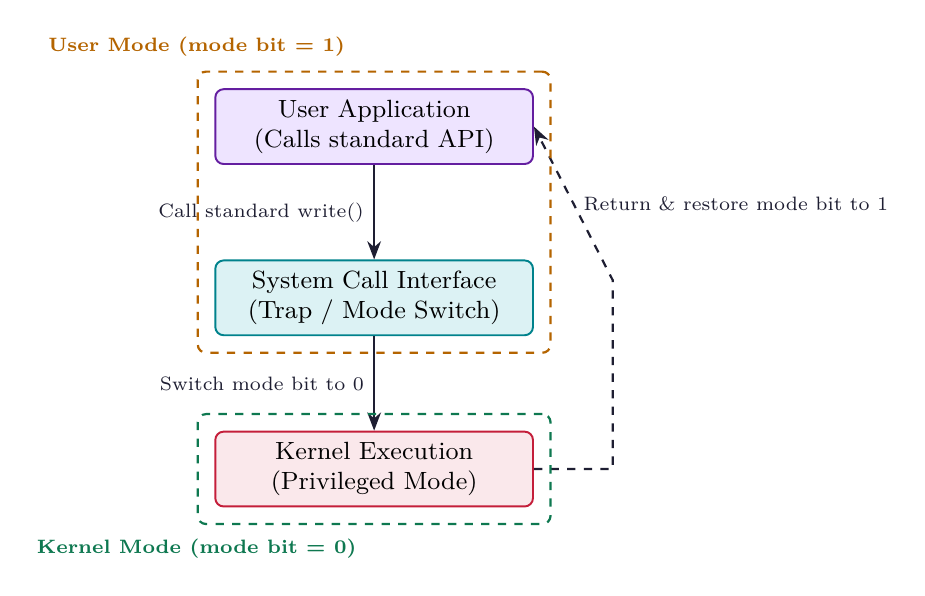
\begin{tikzpicture}[node distance=1.1cm and 2.5cm, thick, font=\small]
  \node[block, text width=3.8cm, fill=hdrpurple, draw=mypurple] (userprog) {User Application\\(Calls standard API)};
  \node[block, text width=3.8cm, fill=hdrteal, draw=myteal, below=1.2cm of userprog] (syscall) {System Call Interface\\(Trap / Mode Switch)};
  \node[block, text width=3.8cm, fill=hdrred, draw=myred, below=1.2cm of syscall] (kernel) {Kernel Execution\\(Privileged Mode)};

  \draw[arrow] (userprog.south) -- node[left, font=\scriptsize] {Call standard write()} (syscall.north);
  \draw[arrow] (syscall.south) -- node[left, font=\scriptsize] {Switch mode bit to 0} (kernel.north);
  \draw[arrow, dashed] (kernel.east) -- ++(1.0, 0) -- ++(0, 2.4) -- node[right, font=\scriptsize] {Return \& restore mode bit to 1} (userprog.east);

  \node[draw=myamber, dashed, inner sep=6pt, rounded corners=3pt, fit=(userprog) (syscall)] (usermode) {};
  \node[font=\scriptsize\bfseries\color{myamber}, above=0.05cm of usermode.north west] {User Mode (mode bit = 1)};
  \node[draw=mygreen, dashed, inner sep=6pt, rounded corners=3pt, fit=(kernel)] (kernelmode) {};
  \node[font=\scriptsize\bfseries\color{mygreen}, below=0.05cm of kernelmode.south west] {Kernel Mode (mode bit = 0)};
\end{tikzpicture}
\end{tcolorbox}

% ===============================================================================
\section{Operating System Architecture Structures}
% ===============================================================================

Operating systems must be structured to ensure reliability, performance, and ease of modification. There are four traditional design methodologies:

\subsection{Monolithic Structure}
In a monolithic operating system, all OS code (scheduling, filesystem, memory management, drivers) runs in a single address space in kernel mode.
\begin{itemize}[leftmargin=*, itemsep=3pt]
  \item \textbf{Advantages:} High performance due to minimal context switching overhead.
  \item \textbf{Disadvantages:} Lack of safety --- a bug in any module (like a camera driver) can crash the entire system.
\end{itemize}

\subsection{Layered Structure}
The OS is broken into a hierarchy of layers (0 to N). Layer 0 is the hardware; Layer N is the user interface.
\begin{itemize}[leftmargin=*, itemsep=3pt]
  \item \textbf{Design Rule:} Each layer is built upon and can only invoke services of lower-level layers.
  \item \textbf{Advantages:} Modular development, simplified debugging.
  \item \textbf{Disadvantages:} Hard to define layers cleanly, and poor performance because each layer crossing introduces execution overhead.
\end{itemize}

\subsection{Microkernel Structure}
The microkernel architecture structures the OS by removing all non-essential components from the kernel, implementing them instead as user-space programs (servers).
\begin{itemize}[leftmargin=*, itemsep=3pt]
  \item \textbf{Core Kernel Services:} Low-level memory management, thread scheduling, and Inter-Process Communication (IPC).
  \item \textbf{Advantages:} High security and reliability. If a filesystem service crashes, the rest of the OS remains unaffected.
  \item \textbf{Disadvantages:} High performance overhead because client programs must communicate with user-space servers via message passing, which requires frequent context switches.
\end{itemize}

\subsection{Hybrid Systems}
Most modern operating systems (e.g., Windows NT, macOS, Linux) use a hybrid design. They combine monolithic speed with microkernel modularity, running core modules in a single address space while using dynamic modules (loadable kernel modules) for extensibility.

\newpage
% ===============================================================================
% MANDATORY QUICK REVISION PAGE
% ===============================================================================
\begin{center}
  {\large\bfseries\color{myred} Quick Revision --- Module 2}\\[3pt]
  {\small\color{mydark} Operating System Structures $|$ OE-EC604B}
\end{center}
\noindent{\color{myred}\rule{\linewidth}{1.2pt}}
\vspace{4pt}

\begin{tcolorbox}[formulabox, title={\textbf{System Call Parameter Passing Methods}}]
\renewcommand{\arraystretch}{1.3}
\begin{tabularx}{\linewidth}{B{3.5cm} X}
Register Method & Parameters passed directly in CPU registers. Fastest, but limited parameter capacity. \\[4pt]
Block / Table Method & Parameters written to a block in memory; pointer to the block is passed in a register. Unlimited size. \\[4pt]
Stack Method & Parameters pushed onto the user stack and popped off by the kernel. Unlimited size.
\end{tabularx}
\tcbset{breakable}
\end{tcolorbox}

\begin{tcolorbox}[defbox, title={\textbf{One-Line Definitions}}]
\begin{itemize}[leftmargin=*, itemsep=2.5pt, topsep=0pt]
  \item \textbf{System Call:} Programmatic request by user-mode applications to execute kernel-mode services.
  \item \textbf{Mode Bit:} A hardware register flag indicating User Mode (1) or Kernel Mode (0).
  \item \textbf{Monolithic Kernel:} OS design where all services run in a single address space inside kernel mode.
  \item \textbf{Microkernel:} Minimalist kernel executing only IPC, scheduling, and basic memory management.
  \item \textbf{Layered Architecture:} Hierarchy of OS layers where layer $i$ relies only on services of layer $i-1$.
  \item \textbf{Trap:} A software-generated interrupt caused by an error or system call request.
  \item \textbf{API (Application Programming Interface):} Standard set of functions wrapper around system calls (e.g., Win32, POSIX).
  \item \textbf{System Program:} File utilities, compilers, or editors that provide a shell wrapper around system calls.
\end{itemize}
\end{tcolorbox}

\begin{tcolorbox}[exambox, title={\textbf{Frequently Asked / Viva Questions}}]
\begin{enumerate}[topsep=0pt, label=\textbf{Q\arabic*.}, itemsep=5pt]
  \item \Q{Why is dual-mode operation supported by hardware in modern operating systems?}
    To protect the system from malicious or poorly written user applications. Privileged instructions (like I/O control or memory protection access) can only be executed in Kernel Mode.
  \item \Q{Describe the sequence of actions that occur when a system call is made.}
    The user program invokes the API function $\to$ API puts system call number in a register $\to$ triggers software interrupt (trap) $\to$ hardware switches mode bit to 0 $\to$ execution jumps to system call handler in kernel $\to$ handler executes kernel code $\to$ mode bit is reset to 1 $\to$ control returns to user program.
  \item \Q{Compare Monolithic Kernels and Microkernels in terms of reliability and performance.}
    Monolithic: High performance (fast function calls, no IPC overhead) but low reliability (any driver crash can bring down the entire OS). Microkernel: High reliability (isolated user-space services) but slower performance (heavy IPC message passing and context switches).
  \item \Q{What are system programs? Give two examples.}
    System programs are user-space utilities that provide a convenient environment for program development and execution. Examples: file command programs (\texttt{cp}, \texttt{mv}) and status utilities (\texttt{ps}, \texttt{top}).
  \item \Q{What are the three common methods used to pass parameters to the operating system during a system call?}
    1. Pass parameters in CPU registers. 2. Store parameters in a memory block/table and pass the block address in a register. 3. Push parameters onto the system stack.
  \item \Q{What is the difference between a system call and a library function?}
    A system call is handled directly by the kernel and involves context switching and privilege escalation. A library function (like \texttt{strlen()}) executes entirely in user mode without kernel intervention.
  \item \Q{Explain the concept of device drivers in OS structure.}
    Device drivers are specialized software modules that translate general I/O commands from the OS kernel into device-specific commands that can be interpreted by hardware controllers.
  \item \Q{Why does the layered architecture model suffer from performance issues?}
    Each layer boundary requires crossing and parameter validation. An application requesting a file read might have to traverse multiple layers sequentially, incurring cumulative overhead.
  \item \Q{What is the POSIX standard?}
    Portable Operating System Interface; a family of standards specified by the IEEE to clarify API compatibility between UNIX-like operating systems.
  \item \Q{How does a hybrid operating system achieve both reliability and speed?}
    By using a monolithic core for speed (running speed-critical elements like graphics and file systems in kernel space) but supporting dynamic loadable kernel modules (LKMs) for driver modularity.
\end{enumerate}
\end{tcolorbox}

\begin{tcolorbox}[tikzbox, title={Comparison of OS Architectures}]
\renewcommand{\arraystretch}{1.4}
\par\noindent
\begin{tabularx}{\linewidth}{|B{2.2cm}|>{\small\centering\arraybackslash}X|>{\small\centering\arraybackslash}X|>{\small\centering\arraybackslash}X|}
\hline
\textbf{Architecture} & \textbf{\color{myred}Context Switch Cost} & \textbf{\color{myteal}Reliability} & \textbf{\color{myamber}Extensibility} \\
\hline
\textbf{Monolithic} & Extremely Low (no IPC) & Poor (no protection) & Hard (requires recompile) \\
\hline
\textbf{Layered} & High (traverses layers) & Moderate & Moderate \\
\hline
\textbf{Microkernel} & Very High (heavy IPC) & Excellent & Very Easy (add user servers) \\
\hline
\end{tabularx}
\end{tcolorbox}


% -- Module 3 -----------------------------------------------------------------
\modulestart{3}{Process Concept and Lifecycle States}

\section{Process Concept and Lifecycle States}
% ===============================================================================

A \textbf{process} is a program in execution. It represents the unit of work in a modern time-sharing system.

\subsection{Process Control Block (PCB)}
Each process is represented in the operating system by a \textbf{Process Control Block (PCB)} (also called a task control block). The PCB contains:
\begin{itemize}[leftmargin=*, itemsep=3pt]
  \item \textbf{Process State:} New, ready, running, waiting, or terminated.
  \item \textbf{Program Counter (PC):} Address of the next instruction to execute.
  \item \textbf{CPU Registers:} Accumulators, index registers, stack pointers.
  \item \textbf{CPU-Scheduling Information:} Process priority, pointers to scheduling queues.
  \item \textbf{Memory-Management Information:} Page tables or segment tables.
  \item \textbf{Accounting Information:} CPU time used, time limits.
  \item \textbf{I/O Status Information:} List of open files, allocated I/O devices.
\end{itemize}

\subsection{Process States and Transitions}

\begin{tcolorbox}[tikzbox, title={Process State Transition Diagram}]
\centering
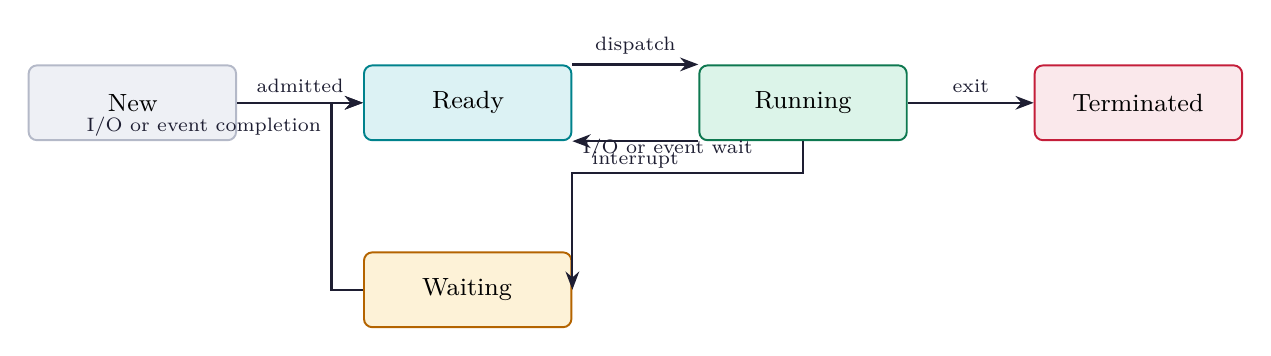
\begin{tikzpicture}[node distance=1.1cm and 1.8cm, thick, font=\small]
  \node[block, fill=hdrgray, draw=mgframe] (new) {New};
  \node[block, right=1.6cm of new, fill=hdrteal, draw=myteal] (ready) {Ready};
  \node[block, right=1.6cm of ready, fill=hdrgreen, draw=mygreen] (running) {Running};
  \node[block, below=1.4cm of ready, fill=hdramber, draw=myamber] (waiting) {Waiting};
  \node[block, right=1.6cm of running, fill=hdrred, draw=myred] (terminated) {Terminated};

  \draw[arrow] (new) -- node[above, font=\scriptsize] {admitted} (ready);
  \draw[arrow] (ready.north east) -- node[above, font=\scriptsize] {dispatch} (running.north west);
  \draw[arrow] (running.south west) -- node[below, font=\scriptsize] {interrupt} (ready.south east);
  \draw[arrow] (running) -- node[above, font=\scriptsize] {exit} (terminated);
  \draw[arrow] (running.south) -- ++(0,-0.4) -| node[right, font=\scriptsize, midway, yshift=0.3cm] {I/O or event wait} (waiting.east);
  \draw[arrow] (waiting.west) -- ++(-0.4,0) |- node[left, font=\scriptsize, midway, yshift=-0.3cm] {I/O or event completion} (ready.west);
\end{tikzpicture}
\end{tcolorbox}

% ===============================================================================
\section{Process Generation \& Scheduling Queues}
% ===============================================================================

\subsection{Process Generation (\texttt{fork()} and \texttt{exec()})}
\begin{itemize}[leftmargin=*, itemsep=3pt]
  \item \textbf{\texttt{fork()} System Call:} Creates a new, child process that is a duplicate of the parent process.
  \begin{itemize}[leftmargin=*, itemsep=2.5pt, topsep=0pt]
    \item In the parent process, \texttt{fork()} returns the PID of the child.
    \item In the child process, \texttt{fork()} returns \texttt{0}.
    \item If the call fails, it returns \texttt{-1}.
  \end{itemize}
  \item \textbf{\texttt{exec()} System Call:} Replaces the process's memory space with a new executable program, changing the active program counter.
\end{itemize}

\subsection{OS Schedulers}
\begin{itemize}[leftmargin=*, itemsep=3pt]
  \item \textbf{Long-Term Scheduler (Job Scheduler):} Selects processes from the pool (disk) and loads them into memory for execution. Controls the \textbf{degree of multiprogramming}.
  \item \textbf{Short-Term Scheduler (CPU Scheduler):} Selects from the processes in memory that are ready to execute and allocates the CPU to one of them. Executes extremely fast.
  \item \textbf{Medium-Term Scheduler:} Temporarily removes processes from memory (swapping) to reduce the degree of multiprogramming and free up RAM.
\end{itemize}

% ===============================================================================
\section{Inter-Process Communication (IPC)}
% ===============================================================================

Processes executing concurrently may be independent or cooperating. Cooperating processes require \textbf{Inter-Process Communication (IPC)}:
1. \textbf{Shared Memory:} A region of memory is established that cooperating processes can read and write to. Fast, but requires manual synchronization to prevent race conditions.
2. \textbf{Message Passing:} Processes exchange messages via the OS kernel without sharing memory space. Easier to implement but slower due to system calls.

% ===============================================================================
\section{Process Synchronization and Critical Section}
% ===============================================================================

A \textbf{race condition} occurs when multiple processes access and manipulate the same data concurrently, and the outcome of the execution depends on the particular order in which the access takes place.

\subsection{The Critical Section Problem}
The \textbf{Critical Section} is a code segment in which a process accesses shared resources.

\begin{tcolorbox}[defbox, title={\textbf{Three Requirements for a Critical Section Solution}}]
1. \textbf{Mutual Exclusion:} If process $P_i$ is executing in its critical section, no other processes can execute in their critical sections.
2. \textbf{Progress:} If no process is executing in its critical section and some processes wish to enter, only those processes not executing in their remainder sections can participate in deciding which process enters next.
3. \textbf{Bounded Waiting:} There must be a limit on the number of times other processes can enter their critical sections after a process has made a request to enter, before that request is granted.
\end{tcolorbox}

\subsection{Semaphores}
A \textbf{Semaphore} is an integer variable $S$ that, apart from initialization, is accessed only through two standard atomic operations: \texttt{wait()} (or P) and \texttt{signal()} (or V).

\begin{tcolorbox}[formulabox, title={\textbf{Semaphore Atomic Implementations}}]
\begin{verbatim}
void wait(Semaphore S) {
    while (S <= 0); // Busy wait (or block process in list)
    S--;
}

void signal(Semaphore S) {
    S++;
}
\end{verbatim}
\begin{itemize}[leftmargin=*, itemsep=3pt]
  \item \textbf{Binary Semaphore (Mutex):} Value can be either 0 or 1. Used for mutual exclusion.
  \item \textbf{Counting Semaphore:} Value ranges over an unrestricted integer domain. Used for resource allocation.
\end{itemize}
\end{tcolorbox}

\subsection{Classical Synchronization Problems}

\subsubsection{Bounded-Buffer (Producer-Consumer) Problem}
Uses semaphores to coordinate a shared buffer of size $N$:
\begin{itemize}[leftmargin=*, itemsep=3pt]
  \item \texttt{mutex} (binary, initial = 1): Protects the buffer insertion/removal.
  \item \texttt{empty} (counting, initial = $N$): Tracks empty buffer slots.
  \item \texttt{full} (counting, initial = 0): Tracks full buffer slots.
\end{itemize}

\subsubsection{Readers-Writers Problem}
Ensures multiple readers can access data concurrently, but only one writer can access it exclusively:
\begin{itemize}[leftmargin=*, itemsep=3pt]
  \item \texttt{rw\_mutex} (binary, initial = 1): Protects critical resource for writers.
  \item \texttt{mutex} (binary, initial = 1): Protects modification of \texttt{read\_count} variable.
\end{itemize}

\subsubsection{Dining Philosophers Problem}
Represents resource allocation challenges among concurrent processes. 5 philosophers sit around a table with 5 chopsticks. Each needs 2 chopsticks to eat. Prone to deadlock if everyone picks up their left chopstick simultaneously.

\subsection{Monitors}
A \textbf{Monitor} is an abstract data type that encapsulates private data and procedures, ensuring that only one process can execute inside the monitor at any given time, preventing synchronization errors automatically.

\newpage
% ===============================================================================
% MANDATORY QUICK REVISION PAGE
% ===============================================================================
\begin{center}
  {\large\bfseries\color{myred} Quick Revision --- Module 3}\\[3pt]
  {\small\color{mydark} Concurrent Processes $|$ OE-EC604B}
\end{center}
\noindent{\color{myred}\rule{\linewidth}{1.2pt}}
\vspace{4pt}

\begin{tcolorbox}[formulabox, title={\textbf{Producer-Consumer Semaphore Code}}]
\begin{tabularx}{\linewidth}{X X}
\textbf{Producer Process:} & \textbf{Consumer Process:} \\
\texttt{do \{} & \texttt{do \{} \\
\texttt{  // produce item} & \texttt{  wait(full);} \\
\texttt{  wait(empty);} & \texttt{  wait(mutex);} \\
\texttt{  wait(mutex);} & \texttt{  // remove item from buffer} \\
\texttt{  // add item to buffer} & \texttt{  signal(mutex);} \\
\texttt{  signal(mutex);} & \texttt{  signal(empty);} \\
\texttt{  signal(full);} & \texttt{  // consume item} \\
\texttt{\} while (true);} & \texttt{\} while (true);}
\end{tabularx}
\end{tcolorbox}

\begin{tcolorbox}[defbox, title={\textbf{One-Line Definitions}}]
\begin{itemize}[leftmargin=*, itemsep=2.5pt, topsep=0pt]
  \item \textbf{Process:} A program in execution containing program counter, stack, data, and registers.
  \item \textbf{PCB:} Process Control Block; kernel data structure storing all attributes of a process.
  \item \textbf{Context Switch:} Saving CPU state of a process and restoring another to switch execution.
  \item \textbf{Race Condition:} State where multiple processes write/read shared data and outcome depends on execution order.
  \item \textbf{Critical Section:} Part of program accessing shared resource that must be protected.
  \item \textbf{Mutual Exclusion:} Preventing more than one process from entering a critical section.
  \item \textbf{Semaphore:} Protected integer variable used for signaling and process synchronization.
  \item \textbf{Monitors:} High-level programming construct providing automated mutual exclusion.
\end{itemize}
\end{tcolorbox}

\begin{tcolorbox}[exambox, title={\textbf{Frequently Asked / Viva Questions}}]
\begin{enumerate}[topsep=0pt, label=\textbf{Q\arabic*.}, itemsep=5pt]
  \item \Q{Draw and label the 5-state process lifecycle model.}
    States: New $\to$ Ready $\to$ Running $\to$ Waiting $\to$ Terminated. Transitions: admitted, scheduler dispatch, interrupt, exit, I/O wait, I/O completion. (See TikZ block diagram).
  \item \Q{What is the difference between fork() and exec() system calls?}
    \texttt{fork()} creates a new duplicate child process with its own PID, copying the parent's memory layout. \texttt{exec()} replaces the current process's entire memory space and code with a new binary program.
  \item \Q{Describe the differences between Long-term, Medium-term, and Short-term schedulers.}
    Long-term: Controls degree of multiprogramming by loading jobs from disk to ready queue (RAM). Short-term: Allocates CPU to a ready process. Medium-term: Performs swapping of processes out of RAM to disk.
  \item \Q{Define a race condition and explain how it can be prevented.}
    A race condition is when multiple processes access and write shared data concurrently and execution order dictates the final value. Prevented by enforcing mutual exclusion using synchronization mechanisms (semaphores, mutex).
  \item \Q{Explain the three criteria that must be satisfied by any solution to the Critical Section problem.}
    1. Mutual Exclusion (only one process inside). 2. Progress (non-critical processes cannot block waiting ones). 3. Bounded Waiting (no starvation, waiting requests must be granted eventually).
  \item \Q{Differentiate between Binary Semaphores and Counting Semaphores.}
    Binary semaphores take values 0 and 1 only, used primarily for mutual exclusion. Counting semaphores take any non-negative integer values, used to manage access to resources with multiple instances.
  \item \Q{What is busy waiting? How do semaphores resolve it?}
    Busy waiting is when a process loops continuously checking a condition (\texttt{while(S <= 0);}), wasting CPU cycles. Resolved by having the semaphore block the process, putting it in a waiting queue and waking it up on \texttt{signal()}.
  \item \Q{Describe the Dining Philosophers synchronization challenge.}
    5 philosophers share 5 chopsticks. If each picks up their left chopstick first, they will all wait indefinitely for their right chopstick, resulting in a deadlock.
  \item \Q{What is a Monitor, and what advantage does it have over raw semaphores?}
    A monitor is a software package encapsulating shared variables and access methods. It ensures mutual exclusion automatically at compile-time/run-time, whereas semaphores are prone to programmer errors (like forgetting a \texttt{signal()} call).
  \item \Q{Why does a context switch introduce performance overhead?}
    Because the CPU must save all register values, program counter, and memory maps of the current process into its PCB, and load those of the new process, during which no useful computation is done.
\end{enumerate}
\end{tcolorbox}

\begin{tcolorbox}[tikzbox, title={IPC Models Comparison}]
\renewcommand{\arraystretch}{1.4}
\par\noindent
\begin{tabularx}{\linewidth}{|B{2.2cm}|>{\small\centering\arraybackslash}X|>{\small\centering\arraybackslash}X|}
\hline
\textbf{Feature} & \textbf{\color{myred}Shared Memory} & \textbf{\color{myteal}Message Passing} \\
\hline
\textbf{Data Transfer Speed} & Extremely Fast (RAM speeds) & Slower (system call overhead) \\
\hline
\textbf{Kernel Involvement} & Only during setup & For every message exchange \\
\hline
\textbf{Synchronization} & Managed by programmer (mutex) & Handled by OS kernel implicitly \\
\hline
\textbf{Use Case} & Large data volume, single machine & Small data volume, distributed systems \\
\hline
\end{tabularx}
\end{tcolorbox}


% -- Module 4 -----------------------------------------------------------------
\modulestart{4}{Scheduling Concepts and Performance Criteria}

\section{Scheduling Concepts and Performance Criteria}
% ===============================================================================

In a single-processor system, only one process can run at a time; others must wait until the CPU is free. The objective of multiprogramming is to run multiple processes concurrently to maximize CPU utilization.

\subsection{CPU-I/O Burst Cycle}
Process execution consists of a cycle of \textbf{CPU execution (CPU burst)} and \textbf{I/O wait (I/O burst)}. Processes alternate between these two states.
\begin{itemize}[leftmargin=*, itemsep=3pt]
  \item \textbf{CPU-bound Process:} Spends most of its time doing computations (long CPU bursts).
  \item \textbf{I/O-bound Process:} Spends most of its time waiting for I/O (short CPU bursts).
\end{itemize}

\subsection{Scheduling Criteria}
Operating systems select processes from the ready queue based on five key performance criteria:
1. \textbf{CPU Utilization:} The percentage of time the CPU is busy executing tasks (Goal: Maximize, 40\% to 90\%).
2. \textbf{Throughput:} The number of processes completed per unit time (Goal: Maximize).
3. \textbf{Turnaround Time ($TAT$):} The total interval from process submission to its completion (Goal: Minimize).
4. \textbf{Waiting Time ($WT$):} The total time a process spends waiting in the ready queue (Goal: Minimize).
5. \textbf{Response Time ($RT$):} The time from submission to the first CPU response (Goal: Minimize, critical for interactive systems).

% ===============================================================================
\section{CPU Scheduling Algorithms}
% ===============================================================================

CPU scheduling decisions take place under four conditions:
1. When a process switches from running to waiting (Non-Preemptive).
2. When a process switches from running to ready (Preemptive).
3. When a process switches from waiting to ready (Preemptive).
4. When a process terminates (Non-Preemptive).

\subsection{First-Come, First-Served (FCFS)}
\begin{itemize}[leftmargin=*, itemsep=3pt]
  \item \textbf{Principle:} The process that requests the CPU first gets it first. Managed via a FIFO queue.
  \item \textbf{Drawback:} Non-preemptive. Suffers from the \textbf{Convoy Effect} --- short processes must wait for a single long process to finish, causing high average waiting times.
\end{itemize}

\subsection{Shortest Job First (SJF)}
\begin{itemize}[leftmargin=*, itemsep=3pt]
  \item \textbf{Principle:} Associates with each process the length of its next CPU burst. The process with the shortest burst is scheduled.
  \item \textbf{SJF (Non-preemptive):} Once CPU is allocated, it cannot be preempted.
  \item \textbf{SRTF (Preemptive SJF):} If a new process arrives with a shorter remaining burst than the currently running process, the CPU is preempted.
  \item \textbf{Advantage:} SJF is \textbf{optimal} --- it gives the minimum average waiting time for a given set of processes.
  \item \textbf{Disadvantage:} Cannot be implemented directly because the length of the next CPU burst is unknown. Prone to \textbf{starvation} of long processes.
\end{itemize}

\subsection{Round Robin (RR) Scheduling}
\begin{itemize}[leftmargin=*, itemsep=3pt]
  \item \textbf{Principle:} Designed for time-sharing systems. The CPU scheduler goes around the ready queue, allocating the CPU to each process for a time interval up to \textbf{1 time quantum (slice)} ($q$).
  \item \textbf{Working:} If process burst $> q$, it is preempted and put back at the tail of the ready queue.
  \item \textbf{Performance Dependency:} If $q$ is extremely large, RR behaves like FCFS. If $q$ is extremely small, it causes high context-switching overhead.
\end{itemize}

\subsection{Priority Scheduling}
\begin{itemize}[leftmargin=*, itemsep=3pt]
  \item \textbf{Principle:} A priority number is associated with each process, and the CPU is allocated to the process with the highest priority (lowest integer usually represents highest priority).
  \item \textbf{Problem:} \textbf{Starvation (Indefinite Blocking)} of low-priority processes.
  \item \textbf{Solution:} \textbf{Aging} --- gradually increasing the priority of processes that wait in the system for a long time.
\end{itemize}

\subsection{Multilevel Queue (MLQ) \& Multilevel Feedback Queue (MLFQ)}
\begin{itemize}[leftmargin=*, itemsep=3pt]
  \item \textbf{MLQ:} Partitioned ready queue into several separate queues (e.g., foreground interactive and background batch) with fixed priority. No movement between queues.
  \item \textbf{MLFQ:} Allows processes to move between queues based on CPU burst history. If a process uses too much CPU time, it is demoted. If it waits too long, it is promoted (aging).
\end{itemize}

\begin{tcolorbox}[tikzbox, title={Multilevel Feedback Queue Structure}]
\centering
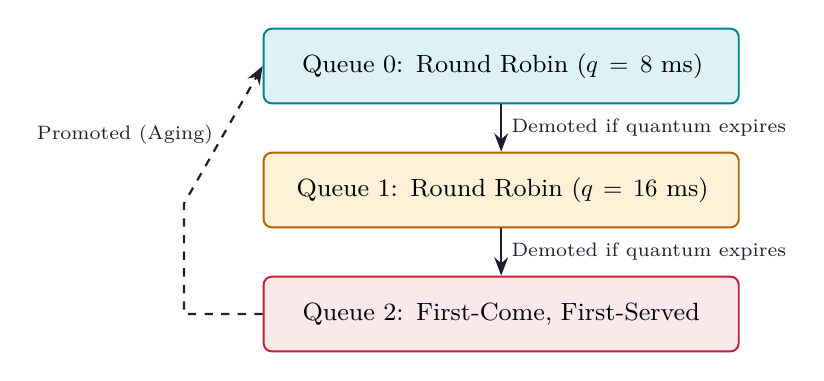
\begin{tikzpicture}[node distance=0.8cm, thick, font=\small]
  \node[block, text width=5.8cm, fill=hdrteal, draw=myteal] (q0) {Queue 0: Round Robin ($q = 8$ ms)};
  \node[block, text width=5.8cm, fill=hdramber, draw=myamber, below=0.6cm of q0] (q1) {Queue 1: Round Robin ($q = 16$ ms)};
  \node[block, text width=5.8cm, fill=hdrred, draw=myred, below=0.6cm of q1] (q2) {Queue 2: First-Come, First-Served};

  \draw[arrow] (q0.south) -- node[right, font=\scriptsize] {Demoted if quantum expires} (q1.north);
  \draw[arrow] (q1.south) -- node[right, font=\scriptsize] {Demoted if quantum expires} (q2.north);
  \draw[arrow, dashed] (q2.west) -- ++(-1.0, 0) -- ++(0, 1.4) -- node[left, font=\scriptsize] {Promoted (Aging)} (q0.west);
\end{tikzpicture}
\end{tcolorbox}

% ===============================================================================
\section{Multiprocessor Scheduling}
% ===============================================================================

When multiple CPUs are available, scheduling complexity increases:
\begin{itemize}[leftmargin=*, itemsep=3pt]
  \item \textbf{Asymmetric Multiprocessing:} One master processor handles all scheduling decisions, I/O processing, and system activities; others run only user code. Simple, but master is a bottleneck.
  \item \textbf{Symmetric Multiprocessing (SMP):} Each processor schedules itself from the common ready queue or private ready queue.
  \item \textbf{Processor Affinity:} A process has an affinity for the processor it is currently running on to avoid the cache invalidation cost of migrating to another CPU.
  \begin{itemize}[leftmargin=*, itemsep=2.5pt, topsep=0pt]
    \item \textbf{Soft Affinity:} OS tries to keep process on same CPU but does not guarantee it.
    \item \textbf{Hard Affinity:} Process specifies it can only run on a subset of CPUs.
  \end{itemize}
  \item \textbf{Load Balancing:} Keeps workload evenly distributed across all CPUs.
  \begin{itemize}[leftmargin=*, itemsep=2.5pt, topsep=0pt]
    \item \textbf{Push Migration:} A specific task monitors load and pushes processes from overloaded CPUs to idle ones.
    \item \textbf{Pull Migration:} An idle processor pulls a waiting task from a busy processor.
    \end{itemize}
  \end{itemize}

\newpage
% ===============================================================================
% MANDATORY QUICK REVISION PAGE
% ===============================================================================
\begin{center}
  {\large\bfseries\color{myred} Quick Revision --- Module 4}\\[3pt]
  {\small\color{mydark} CPU Scheduling $|$ OE-EC604B}
\end{center}
\noindent{\color{myred}\rule{\linewidth}{1.2pt}}
\vspace{4pt}

\begin{tcolorbox}[formulabox, title={\textbf{Core Scheduling Formulas}}]
$$\text{Turnaround Time (TAT)} = \text{Completion Time (CT)} - \text{Arrival Time (AT)}$$
$$\text{Waiting Time (WT)} = \text{Turnaround Time (TAT)} - \text{Burst Time (BT)}$$
$$\text{Response Time (RT)} = \text{First CPU Start Time} - \text{Arrival Time (AT)}$$
$$\text{Average Waiting Time} = \frac{1}{N}\sum_{i=1}^{N} WT_i$$
\end{tcolorbox}

\begin{tcolorbox}[defbox, title={\textbf{One-Line Definitions}}]
\begin{itemize}[leftmargin=*, itemsep=2.5pt, topsep=0pt]
  \item \textbf{Throughput:} Number of completed processes per unit time.
  \item \textbf{Convoy Effect:} Scenario in FCFS where short jobs wait behind a very long job, degrading latency.
  \item \textbf{Preemptive Scheduling:} OS mechanism to interrupt a running process and assign CPU to another.
  \item \textbf{Quantum ($q$):} The fixed time slice allocated to a process in Round Robin scheduling.
  \item \textbf{Starvation:} Situation where a process waits indefinitely because other processes have higher priorities.
  \item \textbf{Aging:} Technique of gradually increasing the priority of waiting processes to prevent starvation.
  \item \textbf{Processor Affinity:} Cache optimization keeping a process executing on the same CPU core.
  \item \textbf{Symmetric Multiprocessing (SMP):} Multiprocessing where each CPU makes its own scheduling decisions.
\end{itemize}
\end{tcolorbox}

\begin{tcolorbox}[exambox, title={\textbf{Frequently Asked / Viva Questions}}]
\begin{enumerate}[topsep=0pt, label=\textbf{Q\arabic*.}, itemsep=5pt]
  \item \Q{Compare FCFS, SJF, and Round Robin scheduling algorithms.}
    FCFS is simple, non-preemptive, but prone to convoy effect. SJF is optimal for average waiting time but causes starvation and is hard to predict. Round Robin is preemptive, quantum-based, and ideal for interactive systems.
  \item \Q{Show the Gantt chart and compute Turnaround and Waiting times for:}\\
    \begin{tabularx}{\linewidth}{|B{1.5cm}|Y|Y|Y|}
    \hline
    Process & Arrival Time & Burst Time & Priority \\
    \hline
    P1 & 0 & 8 & 3 (Low) \\
    P2 & 1 & 4 & 1 (High) \\
    P3 & 2 & 2 & 2 \\
    \hline
    \end{tabularx}\\
    \textbf{Using Preemptive Priority Scheduling:}\par
    \textbf{Gantt Chart:} P1 runs from [0-1]. At $t=1$, P2 arrives with priority 1, preempts P1. P2 runs from [1-5]. At $t=5$, P3 runs from [5-7]. At $t=7$, P1 finishes from [7-14].\par
    \textbf{Completion Times (CT):} P2 = 5, P3 = 7, P1 = 14.\par
    \textbf{Turnaround Times (TAT = CT - AT):} P1 = 14, P2 = 4, P3 = 5. (Avg TAT = 7.67).\par
    \textbf{Waiting Times (WT = TAT - BT):} P1 = 6, P2 = 0, P3 = 3. (Avg WT = 3.0).
  \item \Q{What is the Convoy Effect in CPU scheduling? How is it resolved?}
    It happens in FCFS when one CPU-bound process holds the CPU while multiple I/O-bound processes wait in the ready queue. Resolved by using preemptive scheduling algorithms (like Round Robin).
  \item \Q{Why is SJF scheduling called "optimal"? Why is it difficult to implement?}
    It is optimal because it mathematically minimizes the average waiting time for a set of processes. It is hard to implement because the exact burst time of future processes cannot be known in advance (it must be estimated using exponential smoothing).
  \item \Q{How does the performance of Round Robin scheduling depend on the time quantum?}
    If the quantum is too large, it degenerates into FCFS. If it is too small, it causes excessive context-switching overhead, which wastes CPU cycles. A rule of thumb is that 80\% of CPU bursts should be shorter than the quantum.
  \item \Q{What is starvation? How does aging solve it?}
    Starvation occurs when low-priority processes never get scheduled because high-priority processes keep arriving. Aging solves this by gradually increasing the priority of a process the longer it remains waiting in the ready queue.
  \item \Q{Differentiate between Multilevel Queue (MLQ) and Multilevel Feedback Queue (MLFQ).}
    In MLQ, processes are permanently assigned to a queue based on type, with no queue switching. In MLFQ, processes can move dynamically between queues based on CPU behavior, enabling automatic detection of I/O vs CPU bound jobs.
  \item \Q{Explain Processor Affinity and its types.}
    Processor affinity is the policy of keeping a process on the same CPU to leverage cached data. Soft affinity means the OS tries to enforce this but can migrate the process. Hard affinity guarantees the process runs only on designated CPUs.
  \item \Q{What is the difference between Push and Pull migration in load balancing?}
    Push migration runs a task that periodically checks load and "pushes" processes from busy CPUs to idle ones. Pull migration occurs when an idle CPU queries other CPUs and "pulls" an waiting process to execute.
  \item \Q{Explain CPU-I/O burst cycle.}
    A process's lifecycle alternates between CPU execution blocks (CPU bursts) and waiting for device I/O actions (I/O bursts), ending with a final CPU burst and termination request.
\end{enumerate}
\end{tcolorbox}

\begin{tcolorbox}[tikzbox, title={CPU Scheduling Algorithms Comparison}]
\renewcommand{\arraystretch}{1.4}
\par\noindent
\begin{tabularx}{\linewidth}{|B{2.2cm}|>{\small\centering\arraybackslash}X|>{\small\centering\arraybackslash}X|>{\small\centering\arraybackslash}X|}
\hline
\textbf{Algorithm} & \textbf{\color{myred}Preemptive?} & \textbf{\color{myteal}Starvation Risk?} & \textbf{\color{myamber}Optimal average WT?} \\
\hline
\textbf{FCFS} & No & No & No \\
\hline
\textbf{SJF} & No & Yes & Yes (among non-preemptive) \\
\hline
\textbf{SRTF} & Yes & Yes & Yes (optimal) \\
\hline
\textbf{Round Robin} & Yes & No & No \\
\hline
\textbf{Priority} & Yes/No & Yes & No \\
\hline
\end{tabularx}
\end{tcolorbox}


% -- Module 5 -----------------------------------------------------------------
\modulestart{5}{System Model and Deadlock Characterization}

\section{System Model and Deadlock Characterization}
% ===============================================================================

A \textbf{deadlock} is a state where a set of processes are blocked because each process is holding a resource and waiting for another resource held by some other process in the set.

\subsection{Four Necessary Conditions (Coffman Conditions)}
A deadlock situation can arise if and only if all four of the following conditions hold simultaneously in a system:
1. \textbf{Mutual Exclusion:} At least one resource must be held in a non-shareable mode (only one process can use it at a time).
2. \textbf{Hold and Wait:} A process must be holding at least one resource and waiting to acquire additional resources that are currently being held by other processes.
3. \textbf{No Preemption:} Resources cannot be preempted; a resource can be released only voluntarily by the process holding it, after that process has finished its task.
4. \textbf{Circular Wait:} A closed loop of processes must exist, where each process waits for a resource held by the next process in the loop. E.g., $P_0$ waits for $R_1$ (held by $P_1$), $P_1$ waits for $R_2$ (held by $P_2$), and $P_n$ waits for $R_0$ (held by $P_0$).

\subsection{Resource Allocation Graph (RAG)}
Deadlocks can be described precisely using a directed graph called a \textbf{Resource Allocation Graph (RAG)}:
\begin{itemize}[leftmargin=*, itemsep=3pt]
  \item \textbf{Vertices ($V$):} Divided into two partitions:
  \begin{itemize}[leftmargin=*, itemsep=2.5pt, topsep=0pt]
    \item Processes $P = \{P_1, P_2, \dots, P_n\}$ (represented by circles).
    \item Resource types $R = \{R_1, R_2, \dots, R_m\}$ (represented by rectangles containing dots for instances).
  \end{itemize}
  \item \textbf{Edges ($E$):}
  \begin{itemize}[leftmargin=*, itemsep=2.5pt, topsep=0pt]
    \item \textbf{Request Edge:} Directed edge $P_i \to R_j$ (process $P_i$ has requested resource $R_j$).
    \item \textbf{Assignment Edge:} Directed edge $R_j \to P_i$ (resource instance in $R_j$ is allocated to process $P_i$).
    \end{itemize}
  \end{itemize}

\begin{itemize}[leftmargin=*, itemsep=3pt]
  \item \textbf{Theorem:}
  \begin{itemize}[leftmargin=*, itemsep=2.5pt, topsep=0pt]
    \item If the RAG contains no cycles $\to$ No deadlock.
    \item If the RAG contains a cycle $\to$
      \item If single instance per resource type: Deadlock exists (cycle is necessary and sufficient).
      \item If multiple instances per resource type: Deadlock \textit{may} exist (cycle is necessary but not sufficient).
    \end{itemize}
  \end{itemize}

% ===============================================================================
\section{Deadlock Handling Strategies}
% ===============================================================================

Operating systems use three main strategies to handle deadlocks:

\subsection{1. Deadlock Prevention}
Ensures that the system can never enter a deadlock state by designing the system such that at least one of the four Coffman conditions cannot hold:
\begin{itemize}[leftmargin=*, itemsep=3pt]
  \item \textbf{Prevent Mutual Exclusion:} Make resources shareable (e.g., read-only files). \textbf{Drawback:} Some resources (printers, mutexes) are inherently non-shareable.
  \item \textbf{Prevent Hold and Wait:} Require processes to request all resources at once before execution, or release current resources before requesting new ones. \textbf{Drawback:} Low resource utilization; starvation.
  \item \textbf{Prevent No Preemption:} If a process holding resources requests another that cannot be immediately allocated, all its current resources are preempted (released). \textbf{Drawback:} Overhead of saving/restoring process states.
  \item \textbf{Prevent Circular Wait:} Impose a global ordering on all resource types (e.g., $F(R_j) = i$) and require processes to request resources only in strictly increasing order of enumeration. \textbf{Advantage:} Most practical prevention strategy.
\end{itemize}

\subsection{2. Deadlock Avoidance}
Requires that the OS has prior knowledge of the maximum resources a process will ever request.

\begin{tcolorbox}[defbox, title={\textbf{Safe State vs Unsafe State}}]
A state is \textbf{safe} if there exists a \textbf{safe sequence} $\langle P_1, P_2, \dots, P_n \rangle$ of execution such that, for each $P_i$, the resources that $P_i$ can still request can be satisfied by the currently available resources plus the resources held by all prior processes $P_j$ (for $j < i$).
\end{tcolorbox}

\begin{itemize}[leftmargin=*, itemsep=3pt]
  \item \textbf{Relationship:} A safe state is not deadlocked. An unsafe state is not necessarily deadlocked, but it can lead to a deadlock if processes request their maximum limits. Avoidance algorithms keep the system inside a safe state.
\end{itemize}

\begin{tcolorbox}[tikzbox, title={Deadlock State Space Partitioning}]
\centering
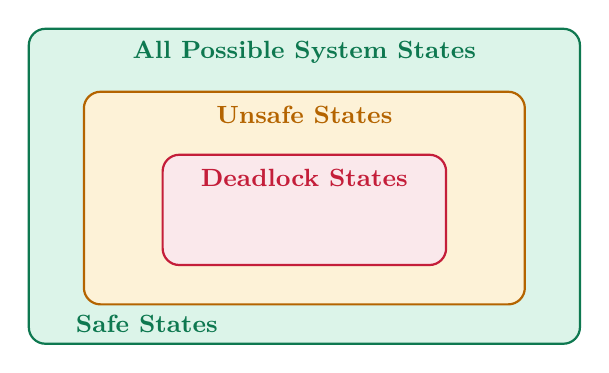
\begin{tikzpicture}[thick, font=\small]
  \draw[draw=mygreen, fill=hdrgreen, rounded corners=6pt] (-3.5, -2.0) rectangle (3.5, 2.0);
  \node[font=\small\bfseries\color{mygreen}] at (0.0, 1.7) {All Possible System States};

  \draw[draw=myamber, fill=hdramber, rounded corners=6pt] (-2.8, -1.5) rectangle (2.8, 1.2);
  \node[font=\small\bfseries\color{myamber}] at (0.0, 0.9) {Unsafe States};

  \draw[draw=myred, fill=hdrred, rounded corners=6pt] (-1.8, -1.0) rectangle (1.8, 0.4);
  \node[font=\small\bfseries\color{myred}] at (0.0, 0.1) {Deadlock States};

  \node[font=\small\bfseries\color{mygreen}] at (-2.0, -1.75) {Safe States};
\end{tikzpicture}
\end{tcolorbox}

\subsubsection{Banker's Algorithm}
Used for systems with multiple instances of resources. Data structures:
\begin{itemize}[leftmargin=*, itemsep=3pt]
  \item \texttt{Available[m]}: Available instances of each resource.
  \item \texttt{Max[n][m]}: Maximum demand of each process.
  \item \texttt{Allocation[n][m]}: Resources currently allocated to each process.
  \item \texttt{Need[n][m]}: Remaining resources a process may request. Note: $\text{Need}[i][j] = \text{Max}[i][j] - \text{Allocation}[i][j]$.
\end{itemize}

\subsection{3. Deadlock Detection \& Recovery}
If a system does not prevent or avoid deadlocks, a deadlock may occur. The OS must provide:
\begin{itemize}[leftmargin=*, itemsep=3pt]
  \item A detection algorithm (periodically runs to find cycles or execute safety checks).
  \item A recovery scheme:
  \begin{itemize}[leftmargin=*, itemsep=2.5pt, topsep=0pt]
    \item \textbf{Process Termination:} Abort all deadlocked processes, or abort one-by-one until the cycle is broken.
    \item \textbf{Resource Preemption:} Preempt resources from some processes, roll back those processes to a safe checkpoint, and restart them.
    \end{itemize}
  \end{itemize}

\newpage
% ===============================================================================
% MANDATORY QUICK REVISION PAGE
% ===============================================================================
\begin{center}
  {\large\bfseries\color{myred} Quick Revision --- Module 5}\\[3pt]
  {\small\color{mydark} Deadlocks $|$ OE-EC604B}
\end{center}
\noindent{\color{myred}\rule{\linewidth}{1.2pt}}
\vspace{4pt}

\begin{tcolorbox}[formulabox, title={\textbf{Banker's Safety Algorithm Equations}}]
Let $\text{Work} = \text{Available}$ and $\text{Finish}[i] = \text{false}$ for $i = 0, 1, \dots, n-1$.
Find an index $i$ such that both:
1. $\text{Finish}[i] == \text{false}$
2. $\text{Need}_i \le \text{Work}$
If such an $i$ exists, update:
$$\text{Work} = \text{Work} + \text{Allocation}_i$$
$$\text{Finish}[i] = \text{true}$$
Repeat. If $\text{Finish}[i] == \text{true}$ for all $i$, the system is in a \textbf{Safe State}.
\end{tcolorbox}

\begin{tcolorbox}[defbox, title={\textbf{One-Line Definitions}}]
\begin{itemize}[leftmargin=*, itemsep=2.5pt, topsep=0pt]
  \item \textbf{Deadlock:} State where processes wait indefinitely for resources held by each other.
  \item \textbf{Mutual Exclusion:} Rule that only one process can hold a resource instance at any time.
  \item \textbf{Hold and Wait:} Process holding resources while requesting more without releasing current ones.
  \item \textbf{Preemption:} Forcible retrieval of allocated resources from a process by the OS.
  \item \textbf{Circular Wait:} Chain of processes where each waits for a resource held by the next.
  \item \textbf{Resource Allocation Graph:} Directed graph showing resource allocations and process requests.
  \item \textbf{Safe Sequence:} Order of process execution that guarantees no deadlock can occur.
  \item \textbf{Ostrich Algorithm:} Deadlock strategy of ignoring the problem (used when deadlocks are rare).
\end{itemize}
\end{tcolorbox}

\begin{tcolorbox}[exambox, title={\textbf{Frequently Asked / Viva Questions}}]
\begin{enumerate}[topsep=0pt, label=\textbf{Q\arabic*.}, itemsep=5pt]
  \item \Q{What are the four necessary conditions for a deadlock to occur?}
    Mutual Exclusion, Hold and Wait, No Preemption, and Circular Wait (Coffman conditions). All four must hold simultaneously for a deadlock to exist.
  \item \Q{Consider a system with 5 processes (P0 to P4) and 3 resource types (A, B, C):}\\
    $\text{Allocation} = \begin{pmatrix} 0 \& 1 \& 0 \\ 2 \& 0 \& 0 \\ 3 \& 0 \& 2 \\ 2 \& 1 \& 1 \\ 0 \& 0 \& 2 \end{pmatrix}, \quad \text{Max} = \begin{pmatrix} 7 \& 5 \& 3 \\ 3 \& 2 \& 2 \\ 9 \& 0 \& 2 \\ 2 \& 2 \& 2 \\ 4 \& 3 \& 3 \end{pmatrix}, \quad \text{Available} = \begin{pmatrix} 3 \& 3 \& 2 \end{pmatrix}$\par
    \textbf{Is the system in a safe state? Find the safe sequence.}\par
    *Step 1: Calculate Need matrix ($\text{Need} = \text{Max} - \text{Allocation}$)*\par
    $\text{Need} = \begin{pmatrix} 7-0 \& 5-1 \& 3-0 \\ 3-2 \& 2-0 \& 2-0 \\ 9-3 \& 0-0 \& 2-2 \\ 2-2 \& 2-1 \& 2-1 \\ 4-0 \& 3-0 \& 3-2 \end{pmatrix} = \begin{pmatrix} 7 \& 4 \& 3 \\ 1 \& 2 \& 2 \\ 6 \& 0 \& 0 \\ 0 \& 1 \& 1 \\ 4 \& 3 \& 1 \end{pmatrix}$\par
    *Step 2: Initialize $\text{Work} = \begin{pmatrix} 3 \& 3 \& 2 \end{pmatrix}$*\par
    \begin{itemize}[leftmargin=*, itemsep=2.5pt, topsep=2pt]
      \item \textbf{Check P1:} $\text{Need}_1 \begin{pmatrix} 1 \& 2 \& 2 \end{pmatrix} \le \text{Work} \begin{pmatrix} 3 \& 3 \& 2 \end{pmatrix}$? Yes. $\text{Work} \to \text{Work} + \text{Alloc}_1 = \begin{pmatrix} 5 \& 3 \& 2 \end{pmatrix}$.
      \item \textbf{Check P3:} $\text{Need}_3 \begin{pmatrix} 0 \& 1 \& 1 \end{pmatrix} \le \text{Work} \begin{pmatrix} 5 \& 3 \& 2 \end{pmatrix}$? Yes. $\text{Work} \to \text{Work} + \text{Alloc}_3 = \begin{pmatrix} 7 \& 4 \& 3 \end{pmatrix}$.
      \item \textbf{Check P0:} $\text{Need}_0 \begin{pmatrix} 7 \& 4 \& 3 \end{pmatrix} \le \text{Work} \begin{pmatrix} 7 \& 4 \& 3 \end{pmatrix}$? Yes. $\text{Work} \to \text{Work} + \text{Alloc}_0 = \begin{pmatrix} 7 \& 5 \& 3 \end{pmatrix}$.
      \item \textbf{Check P2:} $\text{Need}_2 \begin{pmatrix} 6 \& 0 \& 0 \end{pmatrix} \le \text{Work} \begin{pmatrix} 7 \& 5 \& 3 \end{pmatrix}$? Yes. $\text{Work} \to \text{Work} + \text{Alloc}_2 = \begin{pmatrix} 10 \& 5 \& 5 \end{pmatrix}$.
      \item \textbf{Check P4:} $\text{Need}_4 \begin{pmatrix} 4 \& 3 \& 1 \end{pmatrix} \le \text{Work} \begin{pmatrix} 10 \& 5 \& 5 \end{pmatrix}$? Yes. $\text{Work} \to \text{Work} + \text{Alloc}_4 = \begin{pmatrix} 10 \& 5 \& 7 \end{pmatrix}$.
    \end{itemize}
    \textbf{Result:} All processes finished. System is in \textbf{safe state} with safe sequence: $\langle \mathbf{P1, P3, P0, P2, P4} \rangle$.
  \item \Q{Differentiate between Deadlock Prevention and Deadlock Avoidance.}
    Prevention limits system design by enforcing policies that violate one of the 4 Coffman conditions (e.g., resource ordering). Avoidance does not restrict request structures but checks dynamic resource availability and maximum limits to keep the system in a safe state.
  \item \Q{How can the circular wait condition be prevented in operating systems?}
    By defining a global 1-to-1 enumeration function $F: R \to \mathbb{N}$ for all resource types. A process can only request resource $R_j$ if $F(R_j) > F(R_i)$, where $R_i$ is any resource currently held by the process.
  \item \Q{What is an unsafe state? Does it always lead to a deadlock?}
    An unsafe state is a state from which the OS cannot guarantee that all processes can finish their maximum execution. It does \textbf{not} always lead to a deadlock; it will only deadlock if processes actually request their maximum declared resources.
  \item \Q{Why does a cycle in a Resource Allocation Graph (RAG) not always indicate a deadlock?}
    If a resource type has multiple instances, a cycle indicates a potential deadlock but not a guaranteed one, as a process outside the cycle might release an instance, breaking the cycle.
  \item \Q{What is the difference between a Resource Allocation Graph and a Wait-For Graph?}
    A Resource Allocation Graph shows both processes and resources with request/assignment edges. A Wait-For Graph is a simplified version for single-unit resource systems, showing only processes, where edge $P_i \to P_j$ means $P_i$ waits for $P_j$ to release a resource.
  \item \Q{Explain the recovery methods from deadlock.}
    1. Process Termination: Abort all deadlocked processes, or abort processes one-by-one until the cycle is broken. 2. Resource Preemption: Take resources from a process, roll it back to a safe checkpoint, and restart it.
  \item \Q{What is the "Ostrich Algorithm" and when is it appropriate to use?}
    It is the strategy of ignoring deadlocks altogether, assuming they occur rarely. It is used by most general-purpose OS (like Windows/Linux) because deadlock prevention/avoidance adds heavy run-time overhead.
  \item \Q{Why is preemption difficult to implement for some resources?}
    Because some resources (like printers or files being written) cannot be easily saved and restored mid-operation without corrupting data or output.
\end{enumerate}
\end{tcolorbox}

\begin{tcolorbox}[tikzbox, title={Deadlock Handling Trade-offs}]
\renewcommand{\arraystretch}{1.4}
\par\noindent
\begin{tabularx}{\linewidth}{|B{2.2cm}|>{\small\centering\arraybackslash}X|>{\small\centering\arraybackslash}X|>{\small\centering\arraybackslash}X|}
\hline
\textbf{Strategy} & \textbf{\color{myred}Run-time Overhead} & \textbf{\color{myteal}Resource Utilization} & \textbf{\color{myamber}Implementation} \\
\hline
\textbf{Prevention} & None (static rules) & Low (strict limits) & Simple \\
\hline
\textbf{Avoidance} & Moderate (safety checks) & Moderate & Complex (needs max demand) \\
\hline
\textbf{Detection} & High (periodic checks) & High (free allocation) & Moderate \\
\hline
\end{tabularx}
\end{tcolorbox}


% -- Module 6 -----------------------------------------------------------------
\modulestart{6}{Contiguous Memory Allocation}

\section{Contiguous Memory Allocation}
% ===============================================================================

Main memory must accommodate both the operating system and various user processes. In contiguous memory allocation, each process is contained in a single contiguous section of memory.

\subsection{Memory Partitioning Schemes}
\begin{itemize}[leftmargin=*, itemsep=3pt]
  \item \textbf{Fixed Partitioning (MFT - Multiprogramming with a Fixed number of Tasks):} Memory is divided into fixed-size partitions. Each partition contains exactly one process.
  \begin{itemize}[leftmargin=*, itemsep=2.5pt, topsep=0pt]
    \item \textbf{Drawback:} Leads to \textbf{Internal Fragmentation} --- if a process is smaller than the partition allocated to it, the remainder space is wasted.
  \end{itemize}
  \item \textbf{Variable Partitioning (MVT - Multiprogramming with a Variable number of Tasks):} OS maintains a table of free memory slots (holes). When a process arrives, it is allocated a hole matching its size.
  \begin{itemize}[leftmargin=*, itemsep=2.5pt, topsep=0pt]
    \item \textbf{Drawback:} Leads to \textbf{External Fragmentation} --- total free memory is large enough to satisfy a request, but it is not contiguous (split into small holes).
    \item \textbf{Solution:} \textbf{Compaction} --- shifting all processes to one end of memory to group all free holes into a single block (possible only if dynamic relocation is used).
    \end{itemize}
  \end{itemize}

% ===============================================================================
\section{Non-Contiguous Memory Allocation}
% ===============================================================================

To eliminate external fragmentation and the need for compaction, modern systems use non-contiguous memory allocation.

\subsection{Paging Architecture}
\begin{itemize}[leftmargin=*, itemsep=3pt]
  \item \textbf{Frames:} Physical memory is broken into fixed-size blocks (typically $4\,\text{KB}$).
  \item \textbf{Pages:} Logical memory is broken into blocks of the same size.
  \item \textbf{Address Translation:} Every address generated by the CPU is divided into:
  \begin{itemize}[leftmargin=*, itemsep=2.5pt, topsep=0pt]
    \item \textbf{Page Number ($p$):} Used as an index into a \textbf{Page Table} to find the base physical frame.
    \item \textbf{Page Offset ($d$):} Combined with the base frame address to yield the physical address.
    \end{itemize}
  \end{itemize}

\begin{tcolorbox}[tikzbox, title={Paging Hardware Address Translation}]
\centering
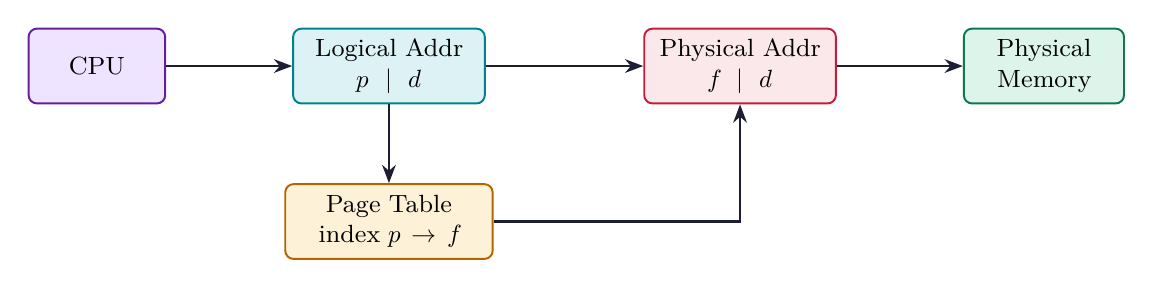
\begin{tikzpicture}[node distance=1.1cm and 2.0cm, thick, font=\small]
  \node[block, text width=1.5cm, fill=hdrpurple, draw=mypurple] (cpu) {CPU};
  \node[block, right=1.6cm of cpu, text width=2.2cm, fill=hdrteal, draw=myteal] (logical) {Logical Addr\\$p \ \ | \ \ d$};
  \node[block, below=1.0cm of logical, text width=2.4cm, fill=hdramber, draw=myamber] (ptable) {Page Table\\index $p \to f$};
  \node[block, right=2.0cm of logical, text width=2.2cm, fill=hdrred, draw=myred] (physical) {Physical Addr\\$f \ \ | \ \ d$};
  \node[block, right=1.6cm of physical, text width=1.8cm, fill=hdrgreen, draw=mygreen] (ram) {Physical\\Memory};

  \draw[arrow] (cpu) -- (logical);
  \draw[arrow] (logical.south) -- ++(0, -0.2) -| (ptable.north);
  \draw[arrow] (ptable.east) -| (physical.south);
  \draw[arrow] (logical.east) -- (physical.west);
  \draw[arrow] (physical) -- (ram);
\end{tikzpicture}
\end{tcolorbox}

\begin{itemize}[leftmargin=*, itemsep=3pt]
  \item \textbf{TLB (Translation Lookaside Buffer):} A fast hardware cache of associative registers used to store recent page-to-frame translations. It reduces the memory access penalty from two cycles (one for page table, one for data) to close to one cycle.
\end{itemize}

\subsection{Segmentation}
Segmentation is a memory-management scheme that supports the programmer's view of memory. A logical address space is a collection of variable-length segments (e.g., main program, procedure, stack, variables).
\begin{itemize}[leftmargin=*, itemsep=3pt]
  \item \textbf{Segment Table:} Maps logical address $\langle \text{segment\_number}, \text{offset} \rangle$ to physical addresses. Each entry has a \textbf{base} (start physical address) and \textbf{limit} (length of segment).
\end{itemize}

% ===============================================================================
\section{Virtual Memory and Demand Paging}
% ===============================================================================

\textbf{Virtual Memory} allows execution of processes that are not completely in main memory. It enables extremely large logical address spaces.

\subsection{Demand Paging \& Page Faults}
Pages are loaded into RAM only when they are referenced during execution (lazy swapper).
\begin{itemize}[leftmargin=*, itemsep=3pt]
  \item \textbf{Page Table Entry:} Includes a \textbf{valid-invalid bit} ($V/I$). $V$ means page is in memory; $I$ means page is on disk.
  \item \textbf{Page Fault:} Occurs when a running process references a page marked as invalid.
  \item \textbf{Page Fault Handling Sequence:}
\end{itemize}
  1. Trap to OS on page fault.
  2. Save process registers and state.
  3. Verify reference is valid, find page location on disk.
  4. Read page from disk into a free frame (using a page replacement algorithm if no free frames exist).
  5. Update page table (set bit to $V$).
  6. Restart the instruction that was interrupted by the trap.

\subsection{Page Replacement Algorithms}
When no frames are free, the OS must swap a page out to make room.
\begin{itemize}[leftmargin=*, itemsep=3pt]
  \item \textbf{FIFO (First-In, First-Out):} Replaces the oldest page. Prone to \textbf{Belady's Anomaly} --- page fault rate increases as physical frame allocation increases.
  \item \textbf{Optimal (OPT):} Replaces the page that will not be used for the longest time in the future. Optimal benchmark, but impossible to implement (requires future knowledge).
  \item \textbf{LRU (Least Recently Used):} Replaces the page that has not been referenced for the longest time in the past. Requires hardware support (counter or stack).
\end{itemize}

\subsection{Thrashing}
\textbf{Thrashing} is a state where a process spends more time paging (swapping pages in and out of disk) than executing useful instructions.
\begin{itemize}[leftmargin=*, itemsep=3pt]
  \item \textbf{Cause:} The process has been allocated fewer frames than its \textbf{working set} (the set of pages it is actively using). As a result, it page faults immediately, forcing page swaps in a continuous loop.
  \item \textbf{Solution:} Working-Set Model (allocates frames based on active page locality) or Page-Fault Frequency (PFF) control.
\end{itemize}

\newpage
% ===============================================================================
% MANDATORY QUICK REVISION PAGE
% ===============================================================================
\begin{center}
  {\large\bfseries\color{myred} Quick Revision --- Module 6}\\[3pt]
  {\small\color{mydark} Memory Management $|$ OE-EC604B}
\end{center}
\noindent{\color{myred}\rule{\linewidth}{1.2pt}}
\vspace{4pt}

\begin{tcolorbox}[formulabox, title={\textbf{Virtual Memory Math}}]
$$\text{Effective Access Time (EAT)} = (1 - p) \times T_{\text{mem}} + p \times T_{\text{fault}}$$
where $p$ = Page Fault Rate ($0 \le p \le 1$), $T_{\text{mem}}$ = RAM Access Time, $T_{\text{fault}}$ = Page Fault Service Time (disk seek + read).
\end{tcolorbox}

\begin{tcolorbox}[defbox, title={\textbf{One-Line Definitions}}]
\begin{itemize}[leftmargin=*, itemsep=2.5pt, topsep=0pt]
  \item \textbf{Internal Fragmentation:} Wasted memory inside a fixed partition allocated to a smaller process.
  \item \textbf{External Fragmentation:} Free memory blocks distributed non-contiguously, preventing allocation.
  \item \textbf{Paging:} Non-contiguous allocation breaking physical memory into fixed frames and logical into pages.
  \item \textbf{TLB:} Translation Lookaside Buffer; hardware cache to speed up logical-to-physical address mapping.
  \item \textbf{Segmentation:} Memory allocation method based on logical units (code, stack, global data).
  \item \textbf{Demand Paging:} Lazy page allocation technique loading pages only on execution references.
  \item \textbf{Belady's Anomaly:} Phenomenon where allocating more physical frames increases page faults in FIFO.
  \item \textbf{Thrashing:} System state where CPUs sit idle because processes are locked in page-swap loops.
\end{itemize}
\end{tcolorbox}

\begin{tcolorbox}[exambox, title={\textbf{Frequently Asked / Viva Questions}}]
\begin{enumerate}[topsep=0pt, label=\textbf{Q\arabic*.}, itemsep=5pt]
  \item \Q{Compare Paging and Segmentation.}
    Paging divides memory into fixed-size blocks (pages/frames), avoiding external fragmentation but suffering from internal fragmentation. It is invisible to the user. Segmentation divides memory into logical variable-size modules, matching the programmer's view, but suffers from external fragmentation.
  \item \Q{Given a reference string: \texttt{7, 0, 1, 2, 0, 3, 0, 4, 2, 3}. Frame size = 3.}\\
    \textbf{Calculate page faults for: (a) FIFO, (b) LRU, (c) Optimal.}\par
    \textbf{(a) FIFO:} Frames status:\par
    \begin{itemize}[leftmargin=*, itemsep=2.5pt, topsep=2pt]
      \item \textbf{Ref 7:} [7] - Fault 1
      \item \textbf{Ref 0:} [7, 0] - Fault 2
      \item \textbf{Ref 1:} [7, 0, 1] - Fault 3
      \item \textbf{Ref 2:} [2, 0, 1] (replaces 7) - Fault 4
      \item \textbf{Ref 0:} [2, 0, 1] - Hit
      \item \textbf{Ref 3:} [2, 3, 1] (replaces 0) - Fault 5
      \item \textbf{Ref 0:} [2, 3, 0] (replaces 1) - Fault 6
      \item \textbf{Ref 4:} [4, 3, 0] (replaces 2) - Fault 7
      \item \textbf{Ref 2:} [4, 2, 0] (replaces 3) - Fault 8
      \item \textbf{Ref 3:} [4, 2, 3] (replaces 0) - Fault 9. \textbf{Total Faults = 9.}
    \end{itemize}
    \textbf{(b) LRU:} Frames status:\par
    \begin{itemize}[leftmargin=*, itemsep=2.5pt, topsep=2pt]
      \item \textbf{Ref 7, 0, 1:} [7, 0, 1] - Faults = 3
      \item \textbf{Ref 2:} [2, 0, 1] (replaces 7) - Fault 4
      \item \textbf{Ref 0:} [2, 0, 1] - Hit (0 is most recent)
      \item \textbf{Ref 3:} [2, 0, 3] (replaces 1) - Fault 5
      \item \textbf{Ref 0:} [2, 0, 3] - Hit
      \item \textbf{Ref 4:} [4, 0, 3] (replaces 2) - Fault 6
      \item \textbf{Ref 2:} [4, 0, 2] (replaces 3) - Fault 7
      \item \textbf{Ref 3:} [3, 0, 2] (replaces 4) - Fault 8. \textbf{Total Faults = 8.}
    \end{itemize}
    \textbf{(c) Optimal:} Frames status:\par
    \begin{itemize}[leftmargin=*, itemsep=2.5pt, topsep=2pt]
      \item \textbf{Ref 7, 0, 1:} [7, 0, 1] - Faults = 3
      \item \textbf{Ref 2:} [2, 0, 1] (replaces 7, unused furthest) - Fault 4
      \item \textbf{Ref 0:} [2, 0, 1] - Hit
      \item \textbf{Ref 3:} [2, 0, 3] (replaces 1, unused furthest) - Fault 5
      \item \textbf{Ref 0:} [2, 0, 3] - Hit
      \item \textbf{Ref 4:} [4, 0, 3] (replaces 2, unused furthest) - Fault 6
      \item \textbf{Ref 2:} [2, 0, 3] (replaces 4) - Fault 7
      \item \textbf{Ref 3:} [2, 0, 3] - Hit. \textbf{Total Faults = 7.}
    \end{itemize}
  \item \Q{What is Belady's Anomaly? Give an example of when it occurs.}
    Belady's Anomaly is when allocating more page frames to a process increases the number of page faults. It occurs in FIFO page replacement. Example string: \texttt{1, 2, 3, 4, 1, 2, 5, 1, 2, 3, 4, 5}. Frame size = 3 gives 9 faults; Frame size = 4 gives 10 faults.
  \item \Q{What is a TLB and how does it improve Effective Access Time?}
    A TLB is a fast associative cache on the CPU containing translation table entries. Instead of doing two memory accesses (one for page table in RAM, one for target location), the CPU checks the TLB. If it's a hit, the translation is resolved in $< 1$ cycle, minimizing EAT.
  \item \Q{Explain the concept of compaction in memory management.}
    Compaction is a technique used to resolve external fragmentation in variable partitioning. The OS dynamically shifts active processes in memory to make them contiguous, merging all small free holes into a single large free partition.
  \item \Q{What is thrashing? How can it be detected and prevented?}
    Thrashing occurs when a process is constantly swapping pages in and out of disk because it has been allocated fewer frames than its active working set. Detected when CPU utilization drops and disk queuing spikes. Prevented using the Working-Set Model or Page-Fault Frequency controls.
  \item \Q{Describe the page fault handling mechanism.}
    Process references page $\to$ MMU detects invalid bit $\to$ traps to OS kernel $\to$ OS checks virtual address and finds page on disk $\to$ allocates free frame $\to$ schedules I/O to read page $\to$ updates page table to valid $\to$ resumes the process.
  \item \Q{How does logical address space differ from physical address space?}
    Logical address space is the set of all virtual addresses generated by a program during compilation/execution. Physical address space is the set of actual physical hardware addresses in main memory (RAM).
  \item \Q{Explain the difference between internal and external fragmentation.}
    Internal fragmentation occurs when allocated memory is slightly larger than the process's demand, leaving wasted space inside the partition. External fragmentation occurs when free memory is sufficient but broken into small, non-contiguous blocks.
  \item \Q{What is a dirty bit (modify bit) and how does it optimize page replacement?}
    A dirty bit is a flag set in the page table entry when a page is written to. During page replacement, if the dirty bit is 0 (page unchanged), the OS can overwrite the frame without writing it back to disk, halving page-fault overhead.
\end{enumerate}
\end{tcolorbox}

\begin{tcolorbox}[tikzbox, title={Page Replacement Algorithms summary}]
\renewcommand{\arraystretch}{1.4}
\par\noindent
\begin{tabularx}{\linewidth}{|B{2.2cm}|>{\small\centering\arraybackslash}X|>{\small\centering\arraybackslash}X|>{\small\centering\arraybackslash}X|}
\hline
\textbf{Algorithm} & \textbf{\color{myred}Implementation Complexity} & \textbf{\color{myteal}Hardware Support?} & \textbf{\color{myamber}Belady's Anomaly?} \\
\hline
\textbf{FIFO} & Very Low & None & Yes \\
\hline
\textbf{Optimal} & Impossible (needs future data) & None & No \\
\hline
\textbf{LRU} & High (requires stacks/counters) & Yes (clock/reference bits) & No \\
\hline
\end{tabularx}
\end{tcolorbox}


% -- Module 7 -----------------------------------------------------------------
\modulestart{7}{I/O Hardware and Organization of I/O Functions}

\section{I/O Hardware and Organization of I/O Functions}
% ===============================================================================

The control of I/O devices connected to the computer is a major function of an operating system. The OS must issue commands to devices, catch interrupts, and handle errors.

\subsection{I/O Communication Methods}
\begin{itemize}[leftmargin=*, itemsep=3pt]
  \item \textbf{Polling (Busy-Wait I/O):} CPU repeatedly reads the status register of the device controller until the device is ready. \textbf{Drawback:} Wastes CPU cycles.
  \item \textbf{Interrupt-Driven I/O:} CPU starts I/O and switches to other tasks. When I/O is ready, the device controller triggers a hardware interrupt, forcing the CPU to branch to the Interrupt Service Routine (ISR).
  \item \textbf{Direct Memory Access (DMA):} Used for high-speed I/O. The DMA controller transfers blocks of data directly between device buffer and main memory, interrupting the CPU only once at the end of the block transfer.
\end{itemize}

\subsection{I/O Buffering}
A buffer is a memory area that stores data temporarily while it is being transferred between two devices or between a device and an application.
\begin{itemize}[leftmargin=*, itemsep=3pt]
  \item \textbf{Single Buffering:} OS assigns a buffer in system memory. The I/O device writes to this buffer, and then the OS copies it to user space.
  \item \textbf{Double Buffering (Ping-Ponging):} OS assigns two buffers. While the user process consumes data from buffer 1, the device writes to buffer 2 in parallel.
  \item \textbf{Circular Buffering:} A queue of three or more buffers used when bursty transfer rates fluctuate.
\end{itemize}

\begin{tcolorbox}[tikzbox, title={Double Buffering Model}]
\centering
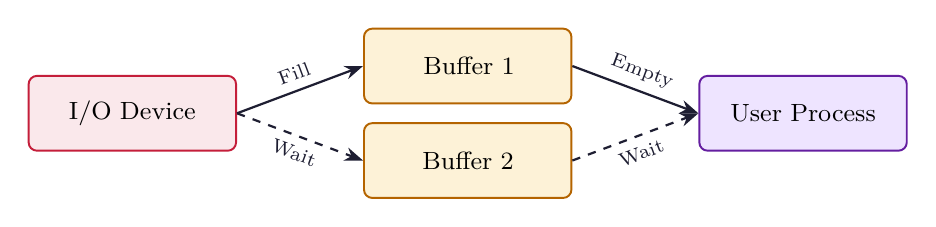
\begin{tikzpicture}[node distance=1.1cm and 1.6cm, thick, font=\small]
  \node[block, fill=hdrred, draw=myred] (dev) {I/O Device};
  \node[block, right=1.6cm of dev, fill=hdramber, draw=myamber, yshift=0.6cm] (buf1) {Buffer 1};
  \node[block, right=1.6cm of dev, fill=hdramber, draw=myamber, yshift=-0.6cm] (buf2) {Buffer 2};
  \node[block, right=1.6cm of buf1, fill=hdrpurple, draw=mypurple, yshift=-0.6cm] (user) {User Process};

  \draw[arrow] (dev.east) -- node[above, font=\scriptsize, sloped] {Fill} (buf1.west);
  \draw[arrow, dashed] (dev.east) -- node[below, font=\scriptsize, sloped] {Wait} (buf2.west);
  \draw[arrow] (buf1.east) -- node[above, font=\scriptsize, sloped] {Empty} (user.west);
  \draw[arrow, dashed] (buf2.east) -- node[below, font=\scriptsize, sloped] {Wait} (user.west);
\end{tikzpicture}
\end{tcolorbox}

% ===============================================================================
\section{Disk Physical Structure and Access Performance}
% ===============================================================================

Magnetic disks provide the bulk of secondary storage for modern systems.
\begin{itemize}[leftmargin=*, itemsep=3pt]
  \item \textbf{Structure:} Disks consist of platters coated with magnetic material. Each platter surface is divided into concentric circles called \textbf{tracks}, which are split into small sectors (typically $512\,\text{Bytes}$). Corresponding tracks on all platters form a \textbf{cylinder}.
  \item \textbf{Disk Access Time:}
  \begin{itemize}[leftmargin=*, itemsep=2.5pt, topsep=0pt]
    \item \textbf{Seek Time ($T_s$):} Time required to move the disk arm to the target cylinder. (Dominates disk latency).
    \item \textbf{Rotational Latency ($T_r$):} Time for the target sector to rotate under the read-write head. (Avg latency = $\frac{1}{2} \times$ time for one rotation).
    \item \textbf{Transfer Time ($T_t$):} Time to actually read/write data. $T_t = \frac{b}{r \cdot N}$ where $b$ = bytes to transfer, $r$ = rotation speed, $N$ = bytes per track.
    \end{itemize}
  \end{itemize}

% ===============================================================================
\section{Disk Scheduling Algorithms}
% ===============================================================================

Because seek time dominates access latency, the OS schedules incoming disk requests to minimize head travel distance.

\subsection*{Request Queue Example}
For the algorithms below, assume a disk with 200 cylinders (0–199). The request queue is:
\texttt{98, 183, 37, 122, 14, 124, 65, 67}. Read-write head starts at cylinder \textbf{53}.

\subsection{First-Come, First-Served (FCFS)}
\begin{itemize}[leftmargin=*, itemsep=3pt]
  \item \textbf{Working:} Services requests in the order of arrival.
  \item \textbf{Head Movement Path:} $53 \to 98 \to 183 \to 37 \to 122 \to 14 \to 124 \to 65 \to 67$.
  \item \textbf{Total head cylinders traversed:} 640. Fair, but very inefficient.
\end{itemize}

\subsection{Shortest Seek Time First (SSTF)}
\begin{itemize}[leftmargin=*, itemsep=3pt]
  \item \textbf{Working:} Selects the request closest to the current head position.
  \item \textbf{Head Movement Path:} $53 \to 65 \to 67 \to 37 \to 14 \to 98 \to 122 \to 124 \to 183$.
  \item \textbf{Total head cylinders traversed:} 236. High efficiency but prone to \textbf{starvation} of outer cylinders.
\end{itemize}

\subsection{SCAN (Elevator Algorithm)}
\begin{itemize}[leftmargin=*, itemsep=3pt]
  \item \textbf{Working:} Arm starts at one end, moves toward the other end, servicing requests, until it reaches the boundary (cylinder 0 or 199), then reverses direction.
  \item \textbf{Head Movement Path (moving towards 0):} $53 \to 37 \to 14 \to \mathbf{0} \to 65 \to 67 \to 98 \to 122 \to 124 \to 183$.
  \item \textbf{Total head cylinders traversed:} 236. Prevents starvation, but treats boundary requests unfairly.
\end{itemize}

\subsection{C-SCAN (Circular SCAN)}
\begin{itemize}[leftmargin=*, itemsep=3pt]
  \item \textbf{Working:} Moves from one end to the other servicing requests. When it reaches the end, it immediately returns to the starting boundary without servicing any requests on the return trip.
  \item \textbf{Head Movement Path (moving towards 199):} $53 \to 65 \to 67 \to 98 \to 122 \to 124 \to 183 \to \mathbf{199} \to \mathbf{0} \to 14 \to 37$.
  \item \textbf{Total head cylinders traversed:} 382. Provides more uniform waiting times.
\end{itemize}

\subsection{LOOK \& C-LOOK}
\begin{itemize}[leftmargin=*, itemsep=3pt]
  \item \textbf{Working:} Similar to SCAN and C-SCAN but the arm goes only as far as the \textbf{last request} in each direction, rather than traveling to the extreme boundaries (0 or 199).
  \item \textbf{C-LOOK Path (moving towards 183):} $53 \to 65 \to 67 \to 98 \to 122 \to 124 \to 183 \to \mathbf{14} \to 37$.
  \item \textbf{Total head cylinders traversed:} 322. Saves travel time compared to C-SCAN.
\end{itemize}

\newpage
% ===============================================================================
% MANDATORY QUICK REVISION PAGE
% ===============================================================================
\begin{center}
  {\large\bfseries\color{myred} Quick Revision --- Module 7}\\[3pt]
  {\small\color{mydark} I/O Management and Disk Scheduling $|$ OE-EC604B}
\end{center}
\noindent{\color{myred}\rule{\linewidth}{1.2pt}}
\vspace{4pt}

\begin{tcolorbox}[formulabox, title={\textbf{Disk Parameter Definitions}}]
$$\text{Total Disk Access Time} = \text{Seek Time} + \text{Rotational Latency} + \text{Transfer Time}$$
$$\text{Average Rotational Latency} = \frac{1}{2} \times \frac{60}{\text{RPM}}\ \text{seconds}$$
\end{tcolorbox}

\begin{tcolorbox}[defbox, title={\textbf{One-Line Definitions}}]
\begin{itemize}[leftmargin=*, itemsep=2.5pt, topsep=0pt]
  \item \textbf{DMA:} Direct Memory Access; I/O technique transferring data blocks to memory without CPU overhead.
  \item \textbf{Double Buffering:} OS buffering model using two registers in parallel to remove consumption stalls.
  \item \textbf{Seek Time:} Time taken for the read-write head assembly to align with the target cylinder.
  \item \textbf{Rotational Latency:} Time taken for the target sector to rotate under the active head.
  \item \textbf{SSTF:} Shortest Seek Time First; scheduling that selects request with minimal seek distance.
  \item \textbf{SCAN:} Elevator scheduling algorithm traversing the entire disk width in cycles.
  \item \textbf{C-SCAN:} Circular SCAN; sweeps in one direction, returning to start instantly without serving.
  \item \textbf{C-LOOK:} SCAN variant that returns immediately after servicing the last request in that direction.
\end{itemize}
\end{tcolorbox}

\begin{tcolorbox}[exambox, title={\textbf{Frequently Asked / Viva Questions}}]
\begin{enumerate}[topsep=0pt, label=\textbf{Q\arabic*.}, itemsep=5pt]
  \item \Q{Explain the difference between Polling, Interrupt-driven I/O, and DMA.}
    Polling has the CPU busy-wait checking status registers. Interrupt-driven I/O triggers hardware interrupts when data is ready, letting the CPU execute other tasks. DMA uses a dedicated controller to transfer large blocks directly between device and memory, interrupting the CPU only once at block completion.
  \item \Q{Compare SCAN, C-SCAN, LOOK, and C-LOOK disk scheduling algorithms.}
    SCAN moves the head to the extreme boundary in one direction, then reverses. C-SCAN goes to the boundary, returns to the other boundary without servicing on the return. LOOK and C-LOOK improve on this by reversing at the last request instead of going to the extreme boundary.
  \item \Q{Give a numerical comparison of SCAN vs LOOK head travel. Head starts at 50 (direction: increasing). Request queue: \texttt{90, 150, 20}. Boundary = 199.}
    \textbf{SCAN:} Head goes $50 \to 90 \to 150 \to \mathbf{199} \to 20$. Head travel: $(199 - 50) + (199 - 20) = 149 + 179 = 328$ cylinders.\par
    \textbf{LOOK:} Head goes $50 \to 90 \to 150 \to 20$ (stops at 150 because it is the last request). Head travel: $(150 - 50) + (150 - 20) = 100 + 130 = 230$ cylinders.
  \item \Q{What is starvation in disk scheduling? Which algorithm is most prone to it?}
    Starvation occurs when a request is never serviced because closer requests keep arriving. SSTF is most prone to starvation because the head tends to stay in localized clusters, leaving requests on the far ends unserviced.
  \item \Q{Explain the mechanical layout of a Hard Disk Drive.}
    A spindle holds multiple circular platters. Read-write heads are mounted on an actuator arm that moves radially. Each platter surface contains concentric tracks, and tracks are divided into sectors. Corresponding tracks vertically form cylinders.
  \item \Q{What is double buffering and why is it preferred over single buffering?}
    Double buffering assigns two buffers. While the CPU reads/empties buffer 1, the device controller fills buffer 2 concurrently. In single buffering, the CPU must stall while the single buffer is being re-filled.
  \item \Q{Define Seek Time, Rotational Latency, and Transfer Time.}
    Seek time is the time to align the arm over the cylinder. Rotational latency is the time for the sector to rotate to the head. Transfer time is the actual data read/write rate.
  \item \Q{A disk rotates at 7200 RPM. What is its average rotational latency?}
    7200 rotations in 60 seconds $\to 1$ rotation takes $60 / 7200 = 8.33\,\text{ms}$. Average rotational latency is half of one rotation time: $0.5 \times 8.33 = 4.17\,\text{ms}$.
  \item \Q{Why does C-SCAN offer more uniform waiting times than SCAN?}
    In SCAN, cylinders near the middle are swept twice as often as those near the boundaries. C-SCAN sweeps in one direction only, returning to start instantly, giving all cylinders a uniform wait interval between sweeps.
  \item \Q{What are the main design issues in I/O system design?}
    Achieving device independence (programs can write to any device without custom code), uniform naming, error handling, buffering optimization, and asynchronous operation.
\end{enumerate}
\end{tcolorbox}

\begin{tcolorbox}[tikzbox, title={Disk Scheduling Algorithms Comparison}]
\renewcommand{\arraystretch}{1.4}
\par\noindent
\begin{tabularx}{\linewidth}{|B{2.2cm}|>{\small\centering\arraybackslash}X|>{\small\centering\arraybackslash}X|>{\small\centering\arraybackslash}X|}
\hline
\textbf{Algorithm} & \textbf{\color{myred}Average Seek Time} & \textbf{\color{myteal}Starvation Risk?} & \textbf{\color{myamber}Boundary Travel?} \\
\hline
\textbf{FCFS} & High (non-optimal) & No & No \\
\hline
\textbf{SSTF} & Low (highly localized) & Yes & No \\
\hline
\textbf{SCAN} & Low & No & Yes (goes to end) \\
\hline
\textbf{C-LOOK} & Low to Moderate & No & No (reverses at last request) \\
\hline
\end{tabularx}
\end{tcolorbox}


% -- Module 8 -----------------------------------------------------------------
\modulestart{8}{File and Directory Concepts}

\section{File and Directory Concepts}
% ===============================================================================

The file system provides the online storage and access mechanism for both data and programs of the operating system.

\subsection{File Concepts \& Access Mechanisms}
\begin{itemize}[leftmargin=*, itemsep=3pt]
  \item \textbf{File Concept:} A file is a named collection of related information that is recorded on secondary storage.
  \item \textbf{Access Methods:}
  \begin{itemize}[leftmargin=*, itemsep=2.5pt, topsep=0pt]
    \item \textbf{Sequential Access:} Information is processed in order, one record after another (e.g., tape storage).
    \item \textbf{Direct (Random) Access:} A file is viewed as a numbered sequence of blocks. The program can read/write any block instantly in any order (e.g., database queries on disk).
    \item \textbf{Indexed Access:} An index table is built containing pointers to various blocks. The program searches the index first to retrieve records.
    \end{itemize}
  \end{itemize}

\subsection{Directory Structures}
A directory is a container that organizes files. Common topologies:
\begin{itemize}[leftmargin=*, itemsep=3pt]
  \item \textbf{Single-Level Directory:} All files are in a single directory. \textbf{Problems:} Naming collisions, organization issues.
  \item \textbf{Two-Level Directory:} Each user gets a private User File Directory (UFD) nested under a Master File Directory (MFD).
  \item \textbf{Tree-Structured Directory:} Users can create subdirectories and organize files hierarchically. The most common structure.
\end{itemize}

\begin{tcolorbox}[tikzbox, title={Tree-Structured Directory Tree}]
\centering
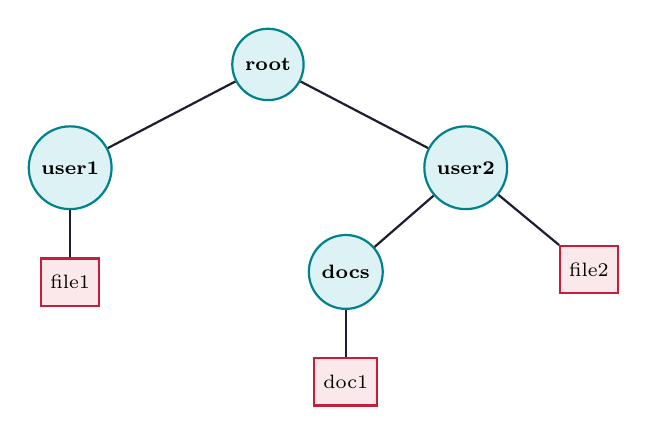
\begin{tikzpicture}[node distance=0.8cm, thick, font=\small,
  dir/.style={circle, draw=myteal, fill=hdrteal, minimum size=0.8cm, font=\scriptsize\bfseries},
  file/.style={rectangle, draw=myred, fill=hdrred, minimum size=0.6cm, font=\scriptsize}]
  \node[dir] (root) {root};
  \node[dir, below left=0.6cm and 1.8cm of root] (user1) {user1};
  \node[dir, below right=0.6cm and 1.8cm of root] (user2) {user2};
  
  \node[file, below=0.6cm of user1] (f1) {file1};
  \node[dir, below left=0.6cm and 0.8cm of user2] (sub) {docs};
  \node[file, below right=0.6cm and 0.8cm of user2] (f2) {file2};
  \node[file, below=0.6cm of sub] (f3) {doc1};

  \draw[line] (root) -- (user1);
  \draw[line] (root) -- (user2);
  \draw[line] (user1) -- (f1);
  \draw[line] (user2) -- (sub);
  \draw[line] (user2) -- (f2);
  \draw[line] (sub) -- (f3);
\end{tikzpicture}
\tcbset{breakable}
\end{tcolorbox}

% ===============================================================================
\section{File System Implementation and Allocation Methods}
% ===============================================================================

To store files on disk, the OS must map logical file blocks to physical disk sectors. There are three traditional allocation methods:

\subsection{1. Contiguous Allocation}
\begin{itemize}[leftmargin=*, itemsep=3pt]
  \item \textbf{Working:} Each file occupies a contiguous set of blocks on the disk.
  \item \textbf{Advantages:} Fast sequential read/write operations because the disk head does not need to move. Easy direct access.
  \item \textbf{Disadvantages:} Prone to \textbf{external fragmentation}. Hard to grow a file dynamically if adjacent blocks are already allocated.
\end{itemize}

\subsection{2. Linked Allocation}
\begin{itemize}[leftmargin=*, itemsep=3pt]
  \item \textbf{Working:} Each file is a linked list of disk blocks. Directory contains a pointer to the first and last blocks of the file. Each block contains a pointer to the next block.
  \item \textbf{Advantages:} No external fragmentation. Files can grow indefinitely.
  \item \textbf{Disadvantages:} Slow random (direct) access (must traverse links sequentially from block 1). Pointers consume storage space. If a pointer gets corrupted, the rest of the file is lost.
  \item \textbf{FAT (File Allocation Table):} A variation of linked allocation. Pointers are stored in a centralized table at the beginning of the volume, caching entries for faster lookup.
\end{itemize}

\subsection{3. Indexed Allocation}
\begin{itemize}[leftmargin=*, itemsep=3pt]
  \item \textbf{Working:} Each file has its own \textbf{index block}, which contains an array of pointers to all its physical data blocks.
  \item \textbf{Advantages:} Supports direct access without traversing lists. No external fragmentation.
  \item \textbf{Disadvantages:} Index block overhead --- wastes space for very small files. If a file grows too large, a single index block is insufficient. (Resolved using linked index blocks, multilevel indexing, or UNIX indirect blocks).
\end{itemize}

% ===============================================================================
\section{Free Space Management}
% ===============================================================================

To allocate blocks, the OS tracks all free disk blocks using one of two common methods:
1. \textbf{Bit Vector (Bit Map):} An array of bits where each bit corresponds to a disk block (0 = allocated, 1 = free). \textbf{Advantages:} Fast, easy to find consecutive blocks. \textbf{Disadvantages:} Must be kept in RAM, consumes space for large disks.
2. \textbf{Linked List:} All free blocks are linked together. Directory keeps a pointer to the first free block. \textbf{Advantages:} Minimal space overhead. \textbf{Disadvantages:} Slow to traverse; hard to find contiguous free blocks.

\newpage
% ===============================================================================
% MANDATORY QUICK REVISION PAGE
% ===============================================================================
\begin{center}
  {\large\bfseries\color{myred} Quick Revision --- Module 8}\\[3pt]
  {\small\color{mydark} File Systems $|$ OE-EC604B}
\end{center}
\noindent{\color{myred}\rule{\linewidth}{1.2pt}}
\vspace{4pt}

\begin{tcolorbox}[formulabox, title={\textbf{File Allocation Calculations}}]
Let block size = $1\,\text{KB}$. Pointer size = $4\,\text{Bytes}$.
\begin{itemize}[leftmargin=*, itemsep=3pt]
  \item \textbf{Single Index Block Limit:} An index block can hold $1\,\text{KB} / 4\,\text{B} = 256$ pointers. Max file size = $256 \times 1\,\text{KB} = 256\,\text{KB}$.
  \item \textbf{Two-Level Indexing Limit:} Primary index block points to 256 secondary index blocks. Max file size = $256 \times 256 \times 1\,\text{KB} = 64\,\text{MB}$.
\end{itemize}
\end{tcolorbox}

\begin{tcolorbox}[defbox, title={\textbf{One-Line Definitions}}]
\begin{itemize}[leftmargin=*, itemsep=2.5pt, topsep=0pt]
  \item \textbf{File:} A named logical collection of related records stored on secondary storage.
  \item \textbf{Sequential Access:} Access method where data is read in sequence from beginning to end.
  \item \textbf{Direct Access:} Random block access where records are accessed directly by block index.
  \item \textbf{Contiguous Allocation:} Allocation method where file blocks are saved in consecutive disk sectors.
  \item \textbf{Linked Allocation:} Allocation method where blocks are linked via pointers in a list structure.
  \item \textbf{FAT:} File Allocation Table; centralized directory indexing system caching linked pointers.
  \item \textbf{Indexed Allocation:} Allocation method where all block pointers are collected in an index block.
  \item \textbf{Bit Vector:} Binary sequence where each bit represents the free/allocated state of a disk block.
\end{itemize}
\end{tcolorbox}

\begin{tcolorbox}[exambox, title={\textbf{Frequently Asked / Viva Questions}}]
\begin{enumerate}[topsep=0pt, label=\textbf{Q\arabic*.}, itemsep=5pt]
  \item \Q{Compare Contiguous, Linked, and Indexed file allocation methods.}
    Contiguous is fast, supports direct access, but suffers from external fragmentation and file-growth limitations. Linked eliminates fragmentation and allows files to grow easily but has slow random access and pointer overhead. Indexed supports direct access and file growth with no fragmentation, but has index block space overhead.
  \item \Q{Explain the FAT (File Allocation Table) file system structure.}
    FAT is a variation of linked allocation. It extracts all block pointers from the data blocks and stores them in a centralized table at the beginning of the partition. The directory entry contains the starting block number, and the table is indexed by block numbers to find subsequent blocks.
  \item \Q{What is an index block in file system implementation? What happens if a file exceeds its capacity?}
    An index block contains an array of disk block addresses allocated to a file. If a file exceeds the index block capacity, the OS uses: 1. Linked scheme (linking multiple index blocks). 2. Multilevel indexing (an index block containing pointers to other index blocks). 3. Combined scheme (like UNIX inodes).
  \item \Q{Describe free space management using a Bit Vector. Calculate the size of a bit map for a 200 GB disk with 4 KB blocks.}
    A bit vector uses 1 bit for each disk block: 1 means free, 0 means allocated.
    \textbf{Total Blocks} = $200\,\text{GB} / 4\,\text{KB} = (200 \times 10^9) / (4 \times 10^3) = 50 \times 10^6$ blocks.\par
    \textbf{Map Size} = $50 \times 10^6$ bits $\approx 6.25\,\text{MB}$ of storage.
  \item \Q{Explain the difference between sequential and direct file access mechanisms.}
    Sequential access processes records one after another from the beginning, moving a read pointer sequentially. Direct access allows reading/writing blocks in any arbitrary order by specifying the relative block number directly.
  \item \Q{What are the advantages of a tree-structured directory over a single-level directory?}
    A tree-structured directory allows users to create nested subdirectories to organize files logically, preventing naming conflicts and enabling file organization, sharing, and access control.
  \item \Q{Explain the implementation issues of contiguous allocation.}
    Finding space for a new file requires executing dynamic allocation algorithms (first-fit, best-fit), which leads to external fragmentation. Also, if a file grows, it may collide with an adjacent allocated file, requiring compaction.
  \item \Q{Why does linked allocation suffer from reliability issues?}
    Because the blocks are scattered across the disk, and each block contains a pointer to the next. If a single sector gets corrupted, the pointer is lost, rendering all subsequent blocks inaccessible.
  \item \Q{What is the purpose of directory mounting?}
    Mounting allows the OS to attach multiple physical file systems on different storage devices (hard disks, USB drives) into a single, unified logical directory tree.
  \item \Q{How does the OS optimize directory lookup speed?}
    By using hash tables or B-trees instead of linear lists to store directory entries, reducing lookup times from $O(N)$ to $O(1)$ or $O(\log N)$.
\end{enumerate}
\end{tcolorbox}

\begin{tcolorbox}[tikzbox, title={File Allocation Methods Comparison}]
\renewcommand{\arraystretch}{1.4}
\par\noindent
\begin{tabularx}{\linewidth}{|B{2.2cm}|>{\small\centering\arraybackslash}X|>{\small\centering\arraybackslash}X|>{\small\centering\arraybackslash}X|}
\hline
\textbf{Feature} & \textbf{\color{myred}Contiguous} & \textbf{\color{myteal}Linked} & \textbf{\color{myamber}Indexed} \\
\hline
\textbf{Direct Access} & Excellent & Very Poor (linear traversal) & Excellent \\
\hline
\textbf{External Frag.} & Yes & None & None \\
\hline
\textbf{Storage Efficiency} & High & Moderate (pointer overhead) & Low for small files \\
\hline
\textbf{File Growth} & Hard (contiguous block) & Easy & Easy \\
\hline
\end{tabularx}
\end{tcolorbox}


% -- Module 9 -----------------------------------------------------------------
\modulestart{9}{Protection \& Security}

\section{Protection \& Security}
% ===============================================================================

Modern computer systems must protect data from unauthorized access, modification, and destruction.
\begin{itemize}[leftmargin=*, itemsep=3pt]
  \item \textbf{Protection:} A mechanism for controlling the access of programs, processes, or users to the resources defined by a computer system.
  \item \textbf{Security:} A measure of confidence that the integrity of a system and its data will be preserved against external threats (viruses, hackers, physical damage).
\end{itemize}

\subsection{Access Matrix Model}
The \textbf{Access Matrix} is a formal protection model. It views the system as a set of \textbf{domains} (active entities, e.g., users, processes) and \textbf{objects} (passive hardware/software components, e.g., files, printers).
\begin{itemize}[leftmargin=*, itemsep=3pt]
  \item \textbf{Grid Entry:} $\text{Matrix}[D, O]$ defines the access rights (read, write, execute) that process in domain $D$ has over object $O$.
  \item \textbf{Implementations:}
  \begin{itemize}[leftmargin=*, itemsep=2.5pt, topsep=0pt]
    \item \textbf{Access Control List (ACL):} Associates with each object a list of domains and their permitted rights (columns of the matrix). Used in Unix/Windows filesystems.
    \item \textbf{Capability List (C-List):} Associates with each domain a list of objects and rights (rows of the matrix).
    \end{itemize}
  \end{itemize}

% ===============================================================================
\section{Introduction to Distributed Operating Systems}
% ===============================================================================

A \textbf{Distributed Operating System} manages a collection of independent, networked, and physically separate computational nodes, presenting them to the user as a single, unified computer system.
\begin{itemize}[leftmargin=*, itemsep=3pt]
  \item \textbf{Network OS vs. Distributed OS:} In a Network OS, users are aware of the existence of multiple computers (e.g., must use \texttt{ssh} or remote mounting). A Distributed OS provides \textbf{location transparency} --- the user cannot tell where a program is running or where a file is stored.
\end{itemize}

% ===============================================================================
\section{Case Study: The UNIX Operating System}
% ===============================================================================

UNIX is a highly modular, multitasking operating system originally developed at Bell Labs.

\subsection{System Architecture}
UNIX is divided into three main layers:
1. \textbf{User Space:} Applications, library calls, and the command interpreter (Shell).
2. \textbf{Kernel Space:} Manages process execution, memory, file systems, interrupts, and I/O.
3. \textbf{Hardware:} The underlying CPU, memory, and physical controllers.

\subsection{The UNIX File System (Inode Structure)}
In UNIX, every file is represented by a data structure called an \textbf{Inode (Index Node)}. The inode contains file metadata (owner, permissions, size, time stamps) and a table of \textbf{block addresses} pointing to the physical data on disk.

\begin{itemize}[leftmargin=*, itemsep=3pt]
  \item \textbf{Inode Address Pointers Layout:} Typically contains 15 pointers:
  \begin{itemize}[leftmargin=*, itemsep=2.5pt, topsep=0pt]
    \item \textbf{Pointers 0–11:} \textbf{Direct Blocks} (point directly to disk data blocks).
    \item \textbf{Pointer 12:} \textbf{Single Indirect Block} (points to a block containing pointers to data blocks).
    \item \textbf{Pointer 13:} \textbf{Double Indirect Block} (points to a block containing pointers to single indirect blocks).
    \item \textbf{Pointer 14:} \textbf{Triple Indirect Block} (points to a block containing pointers to double indirect blocks).
    \end{itemize}
  \end{itemize}

\begin{tcolorbox}[tikzbox, title={UNIX Inode Block Mapping Architecture}]
\centering
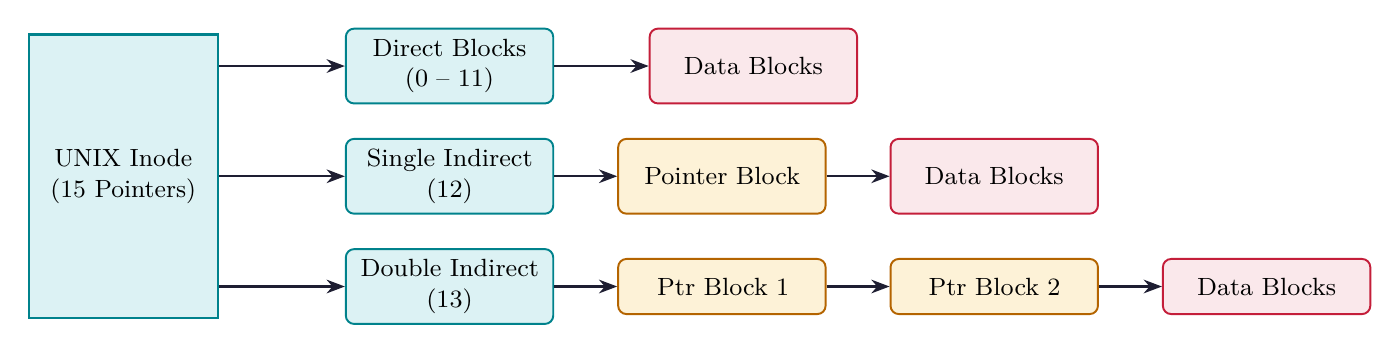
\begin{tikzpicture}[node distance=0.6cm and 1.8cm, thick, font=\small]
  % Inode
  \node[draw=myteal, fill=hdrteal, minimum width=2.4cm, minimum height=3.6cm, align=center] (inode) {UNIX Inode\\(15 Pointers)};
  
  % Direct Blocks
  \node[block, right=1.6cm of inode, yshift=1.4cm] (direct) {Direct Blocks\\(0 -- 11)};
  \node[block, right=1.2cm of direct, fill=hdrred, draw=myred] (db) {Data Blocks};
  
  % Single Indirect
  \node[block, right=1.6cm of inode, yshift=0.0cm] (ind1) {Single Indirect\\(12)};
  \node[block, right=0.8cm of ind1, fill=hdramber, draw=myamber] (pt1) {Pointer Block};
  \node[block, right=0.8cm of pt1, fill=hdrred, draw=myred] (db2) {Data Blocks};
  
  % Double Indirect
  \node[block, right=1.6cm of inode, yshift=-1.4cm] (ind2) {Double Indirect\\(13)};
  \node[block, right=0.8cm of ind2, fill=hdramber, draw=myamber, minimum height=0.7cm] (pt2) {Ptr Block 1};
  \node[block, right=0.8cm of pt2, fill=hdramber, draw=myamber, minimum height=0.7cm] (pt3) {Ptr Block 2};
  \node[block, right=0.8cm of pt3, fill=hdrred, draw=myred, minimum height=0.7cm] (db3) {Data Blocks};

  \draw[arrow] (inode.east |- direct.west) -- (direct.west);
  \draw[arrow] (direct.east) -- (db.west);
  
  \draw[arrow] (inode.east) -- (ind1.west);
  \draw[arrow] (ind1.east) -- (pt1.west);
  \draw[arrow] (pt1.east) -- (db2.west);
  
  \draw[arrow] (inode.east |- ind2.west) -- (ind2.west);
  \draw[arrow] (ind2.east) -- (pt2.west);
  \draw[arrow] (pt2.east) -- (pt3.west);
  \draw[arrow] (pt3.east) -- (db3.west);
\end{tikzpicture}
\end{tcolorbox}

\subsection{UNIX Process Management \& Scheduling}
\begin{itemize}[leftmargin=*, itemsep=3pt]
  \item \textbf{Process Creation:} Handled exclusively via \texttt{fork()} followed by \texttt{exec()}.
  \item \textbf{UNIX Process States:} Running in user mode, Running in kernel mode, Ready to run in memory, Asleep in memory (waiting for I/O), Ready to run swapped, Asleep swapped, Zombie (terminated but parent has not read exit status).
  \item \textbf{UNIX CPU Scheduling:} Uses a multilevel feedback queue scheduling algorithm. Priority is recalculated every second based on CPU usage:
\end{itemize}
$$\text{Priority} = \text{Base} + \frac{\text{Recent CPU Usage}}{2} + \text{Nice}$$
where \texttt{Nice} is a user-controllable process parameter (higher \texttt{Nice} value lowers priority).

\newpage
% ===============================================================================
% MANDATORY QUICK REVISION PAGE
% ===============================================================================
\begin{center}
  {\large\bfseries\color{myred} Quick Revision --- Module 9}\\[3pt]
  {\small\color{mydark} Protection, Security and UNIX Case Study $|$ OE-EC604B}
\end{center}
\noindent{\color{myred}\rule{\linewidth}{1.2pt}}
\vspace{4pt}

\begin{tcolorbox}[formulabox, title={\textbf{UNIX Inode Max File Size Calculations}}]
Let block size = $1\,\text{KB}$. Disk address pointer = $4\,\text{Bytes}$.
\begin{itemize}[leftmargin=*, itemsep=3pt]
  \item \textbf{Max Direct Blocks Capacity:} $12 \times 1\,\text{KB} = 12\,\text{KB}$.
  \item \textbf{Max Single Indirect Capacity:} $(1\,\text{KB} / 4\,\text{B}) \times 1\,\text{KB} = 256 \times 1\,\text{KB} = 256\,\text{KB}$.
  \item \textbf{Max Double Indirect Capacity:} $256 \times 256 \times 1\,\text{KB} = 64\,\text{MB}$.
  \item \textbf{Max Triple Indirect Capacity:} $256 \times 256 \times 256 \times 1\,\text{KB} = 16\,\text{GB}$.
  \item \textbf{Total Max File Size Limit:} $12\,\text{KB} + 256\,\text{KB} + 64\,\text{MB} + 16\,\text{GB} \approx 16.06\,\text{GB}$.
\end{itemize}
\end{tcolorbox}

\begin{tcolorbox}[defbox, title={\textbf{One-Line Definitions}}]
\begin{itemize}[leftmargin=*, itemsep=2.5pt, topsep=0pt]
  \item \textbf{Access Matrix:} Grid model representing domains (rows), objects (columns), and access rights (cells).
  \item \textbf{ACL:} Access Control List; column-wise access matrix stored on objects indicating permitted domains.
  \item \textbf{Capability List:} Row-wise access matrix stored inside process domains detailing object rights.
  \item \textbf{Distributed OS:} OS presenting multiple physical CPU nodes as a single logical computer transparently.
  \item \textbf{Location Transparency:} File or computation access method independent of physical node location.
  \item \textbf{Superblock:} UNIX filesystem metadata block containing system size, free block count, and inode limits.
  \item \textbf{UNIX Inode:} Index block detailing metadata and 15 storage pointers for a UNIX file.
  \item \textbf{Zombie Process:} Process that has terminated but still occupies an entry in the process table.
\end{itemize}
\end{tcolorbox}

\begin{tcolorbox}[exambox, title={\textbf{Frequently Asked / Viva Questions}}]
\begin{enumerate}[topsep=0pt, label=\textbf{Q\arabic*.}, itemsep=5pt]
  \item \Q{Differentiate between Protection and Security in operating systems.}
    Protection is the internal OS mechanism to control process/user access to defined system resources. Security is the external defense mechanism protecting system integrity and data against threats like malware, hackers, and environment disasters.
  \item \Q{Compare Access Control Lists (ACLs) and Capability Lists (C-Lists).}
    ACLs are column-oriented implementations of the Access Matrix; they associate permitted domains and rights directly with each object (e.g., file permissions). C-Lists are row-oriented; they attach object rights to each domain/user process directly.
  \item \Q{What is a Distributed Operating System? What are its primary advantages?}
    A Distributed OS coordinates multiple autonomous CPUs connected by communication networks, presenting them as a single logical machine. Advantages include resource sharing, computational speedup, reliability (fault tolerance), and scalability.
  \item \Q{Explain the UNIX Inode pointer layout and calculate max file size for a 2 KB block size with 4-byte pointers.}
    Layout has 12 direct, 1 single indirect, 1 double indirect, and 1 triple indirect pointers.
    \textbf{Pointers per block} = $2\,\text{KB} / 4\,\text{B} = 512$.\par
    \textbf{Direct size} = $12 \times 2\,\text{KB} = 24\,\text{KB}$.\par
    \textbf{Single indirect size} = $512 \times 2\,\text{KB} = 1024\,\text{KB} = 1\,\text{MB}$.\par
    \textbf{Double indirect size} = $512^2 \times 2\,\text{KB} = 512\,\text{MB}$.\par
    \textbf{Triple indirect size} = $512^3 \times 2\,\text{KB} = 256\,\text{GB}$.\par
    \textbf{Max File Size} = $24\,\text{KB} + 1\,\text{MB} + 512\,\text{MB} + 256\,\text{GB} \approx 256.5\,\text{GB}$.
  \item \Q{What is the function of the Superblock in the UNIX file system?}
    The Superblock is located at a fixed offset near the start of the disk partition. It contains critical metadata about the file system, including total blocks, free block count, free inode list, size of inode list, and status flag.
  \item \Q{Describe the UNIX process scheduling formula and explain the role of the nice value.}
    $\text{Priority} = \text{Base} + (\text{Recent CPU Usage} / 2) + \text{Nice}$. The OS decays priority based on CPU usage to prevent CPU starvation. The \texttt{Nice} value is an administrator/user offset (ranging from $-20$ to $+19$). A higher nice value increases the priority value, which actually lowers scheduling priority.
  \item \Q{What is a zombie process in UNIX? How is it cleared?}
    A zombie process is a process that has finished execution but still has an entry in the system process table to allow its parent to read its exit code (via \texttt{wait()}). It is cleared when the parent executes a \texttt{wait()} system call. If the parent terminates, the zombie is inherited by the \texttt{init} process, which automatically calls \texttt{wait()}.
  \item \Q{Differentiate between Loosely Coupled and Tightly Coupled distributed systems.}
    Loosely coupled systems have independent nodes with private memory connected via slow communication networks (e.g., LAN clusters). Tightly coupled systems share a common physical memory and bus architecture with fast inter-processor communication.
  \item \Q{What is the Access Matrix model? How is it represented?}
    It is a security model where rows represent domains, columns represent objects, and cell entries represent the set of access rights (read, write, execute) allowed for a domain over an object.
  \item \Q{Explain the role of the shell in the UNIX operating system.}
    The shell is a user-space application that acts as a command line interpreter, reading user commands, expanding wildcards, setting up I/O redirection/piping, and spawning processes using \texttt{fork}/\texttt{exec} to execute those commands.
\end{enumerate}
\end{tcolorbox}

\begin{tcolorbox}[tikzbox, title={Security Implementation Comparison}]
\renewcommand{\arraystretch}{1.4}
\par\noindent
\begin{tabularx}{\linewidth}{|B{2.2cm}|>{\small\centering\arraybackslash}X|>{\small\centering\arraybackslash}X|}
\hline
\textbf{Feature} & \textbf{\color{myred}Access Control List (ACL)} & \textbf{\color{myteal}Capability List (C-List)} \\
\hline
\textbf{Association} & Attached to the Object (e.g. File) & Attached to the Subject (e.g. Domain) \\
\hline
\textbf{Revocation} & Easy (just delete domain from file list) & Hard (must search all domain lists) \\
\hline
\textbf{Access check} & Slow (must search file ACL at access) & Fast (domain presents token directly) \\
\hline
\textbf{Common use} & Standard OS filesystems & Object-oriented/microkernel systems \\
\hline
\end{tabularx}
\end{tcolorbox}


\end{document}
